\chapter{Growth yield analysis}
\label{chap:yield_analysis}

Chapters~\ref{chap:growth} and \ref{chap:properties} showed how the \hkl{1 1 1} facet stabilisation method affects the internal composition and morphology of nanowires grown with the \acf{tase} process. These results, obtained on \hkl(0 0 1) and \hkl(1 1 0) \acf{soi} wafers with different device layer thicknesses, showed reliable growth rates and structural results. However, a quantitative analysis of this growth method's yield is needed to understand its success rate better. 

This chapter presents the research my co-authors and I carried out and published in \cite{Brugnolotto2023_2, Brugnolotto2024}. The structure and appearance of the surface of samples 6 and 7 is described. The assumption of correlation between the internal structure seen with \acf{stem_m} and the top-down low-resolution data collected with \acf{sem_m} is explained. A statistical analysis that compares the wires between perfectly grown and defective and evaluates the impact of parasitic crystal growth is presented, involving \num{15840} wires equally divided between the two abovementioned samples. 

The second half of the chapter focuses on using the dataset containing \num{240} \acs{sem_m} images as input data for the supervised training of a machine learning algorithm for automatically classifying wires. Using digital image processing, a strategy is presented to isolate each single wire from the \num{240} arrays. The ability to create single-wire images enables the use of a lightweight image classifier. Finally, the performance of the splitting algorithm and the resulting classifier are examined, together with some improvements to the former.

\section{Sample characteristics}

\begin{figure}
    \centering
    \subcaptionbox{
        Mask of a single array.
        \label{subfig:mask_array}
    }{
        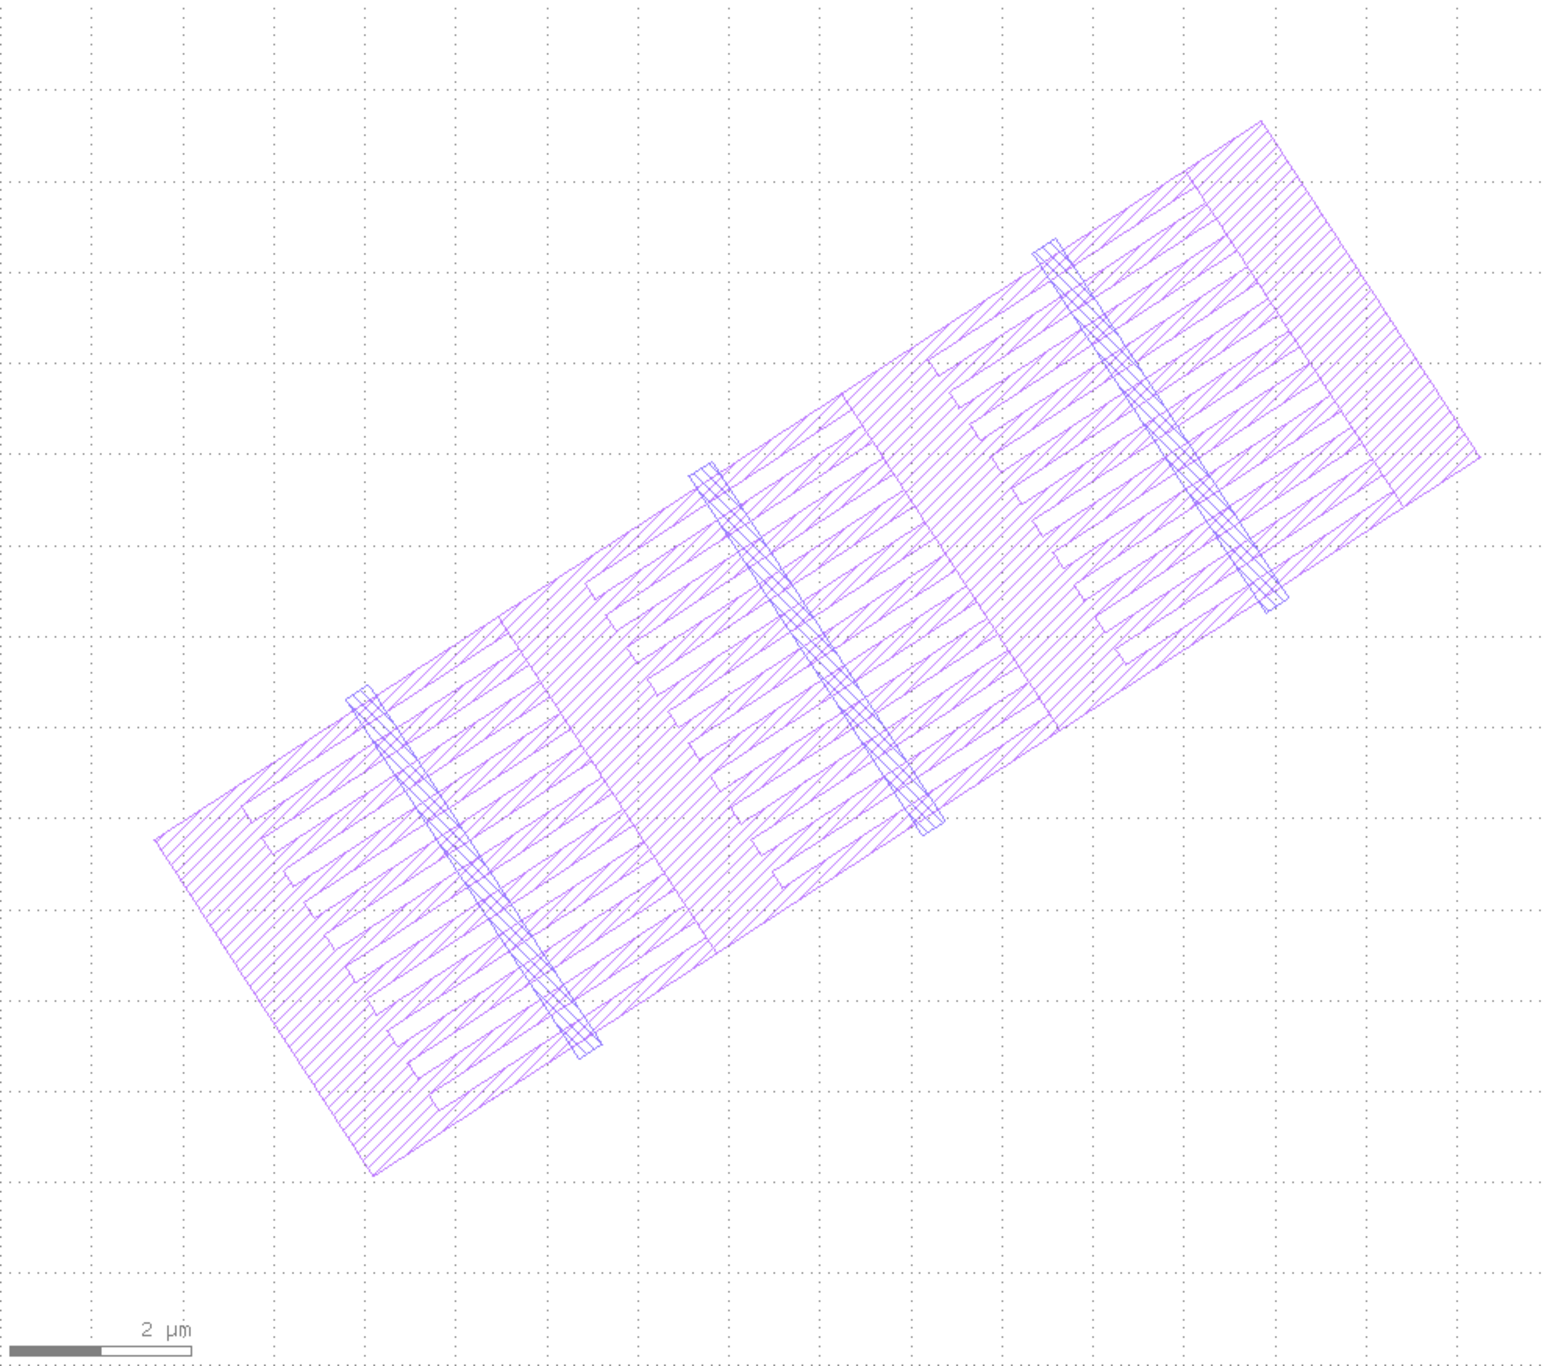
\includegraphics[width = 0.48\textwidth]{5_Yield_Analysis/Fig/mask_array.pdf}
    }
    \subcaptionbox{
        Mask of a section of the chip.
        \label{subfig:mask_section}
    }{
        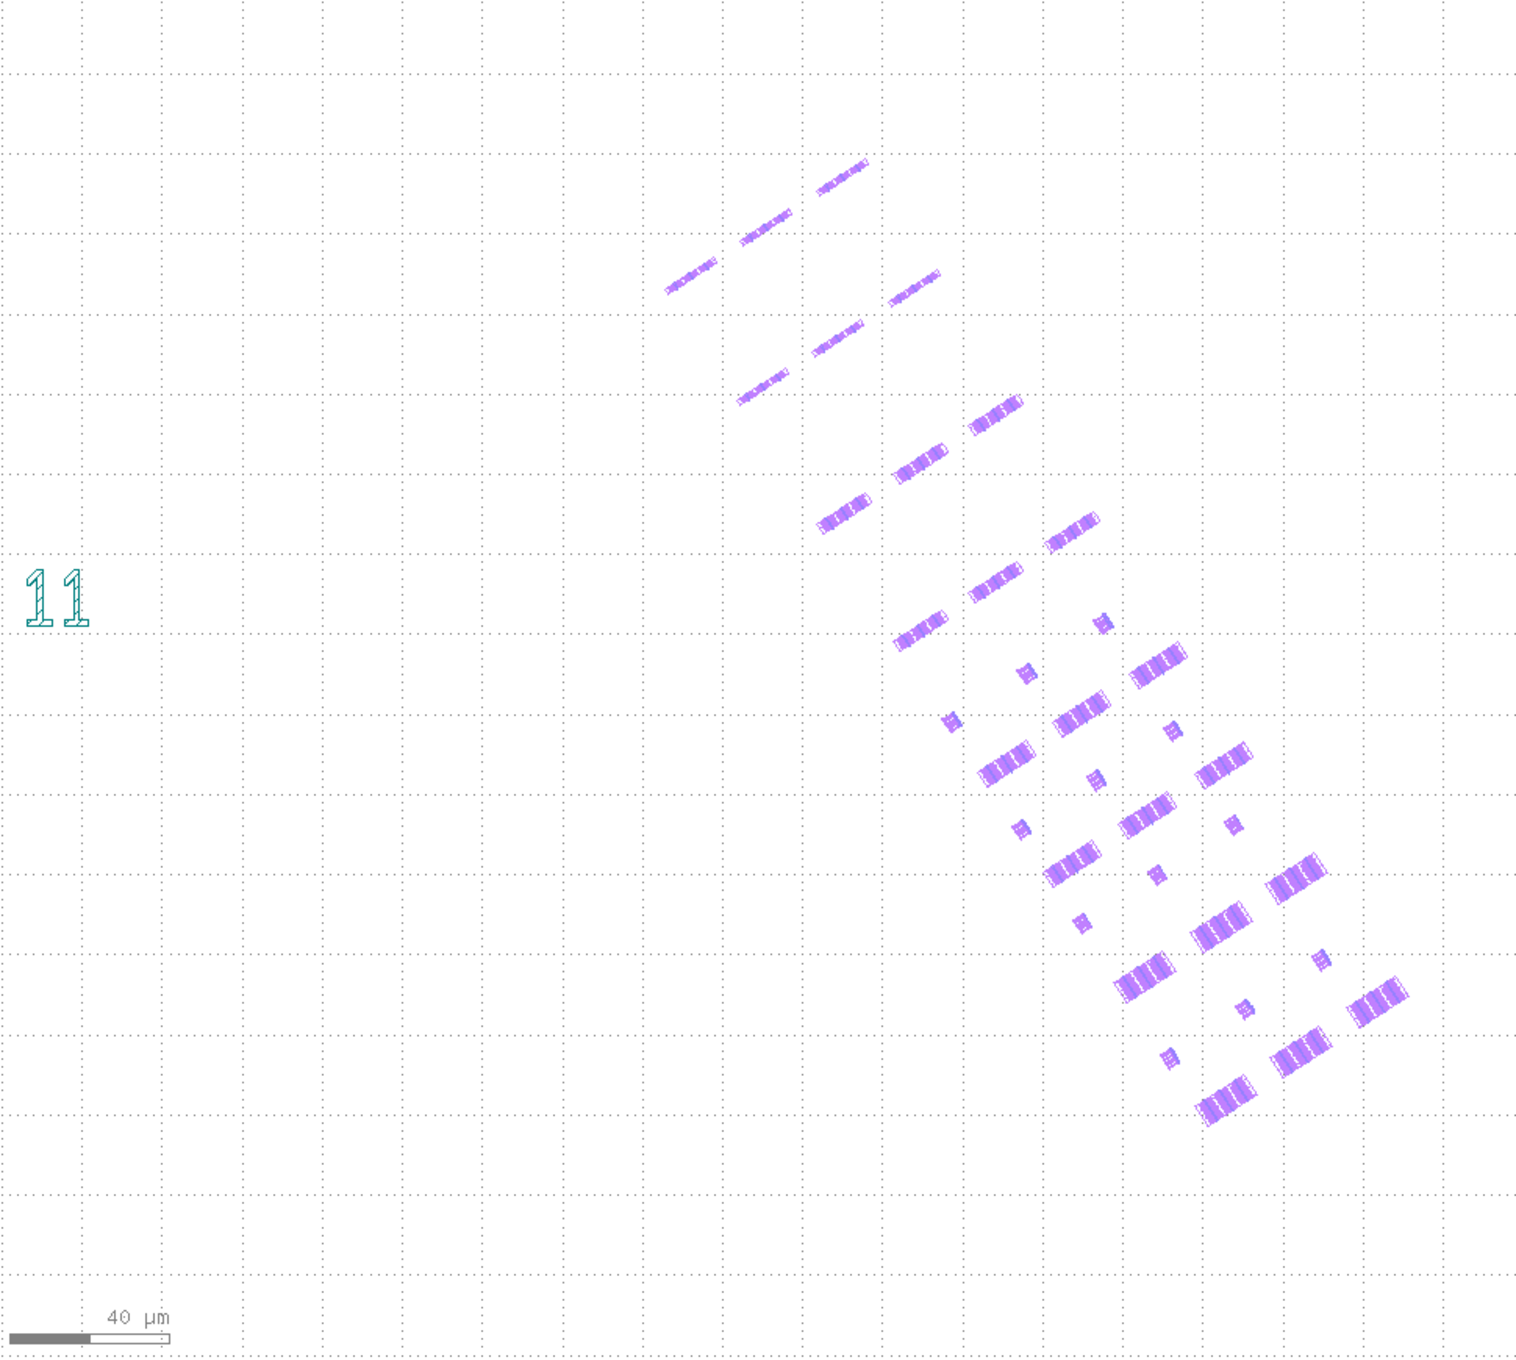
\includegraphics[width = 0.48\textwidth]{5_Yield_Analysis/Fig/mask_section.pdf}
    }
    \subcaptionbox{
        Mask of a division of the chip.
        \label{subfig:mask_division}
    }{
        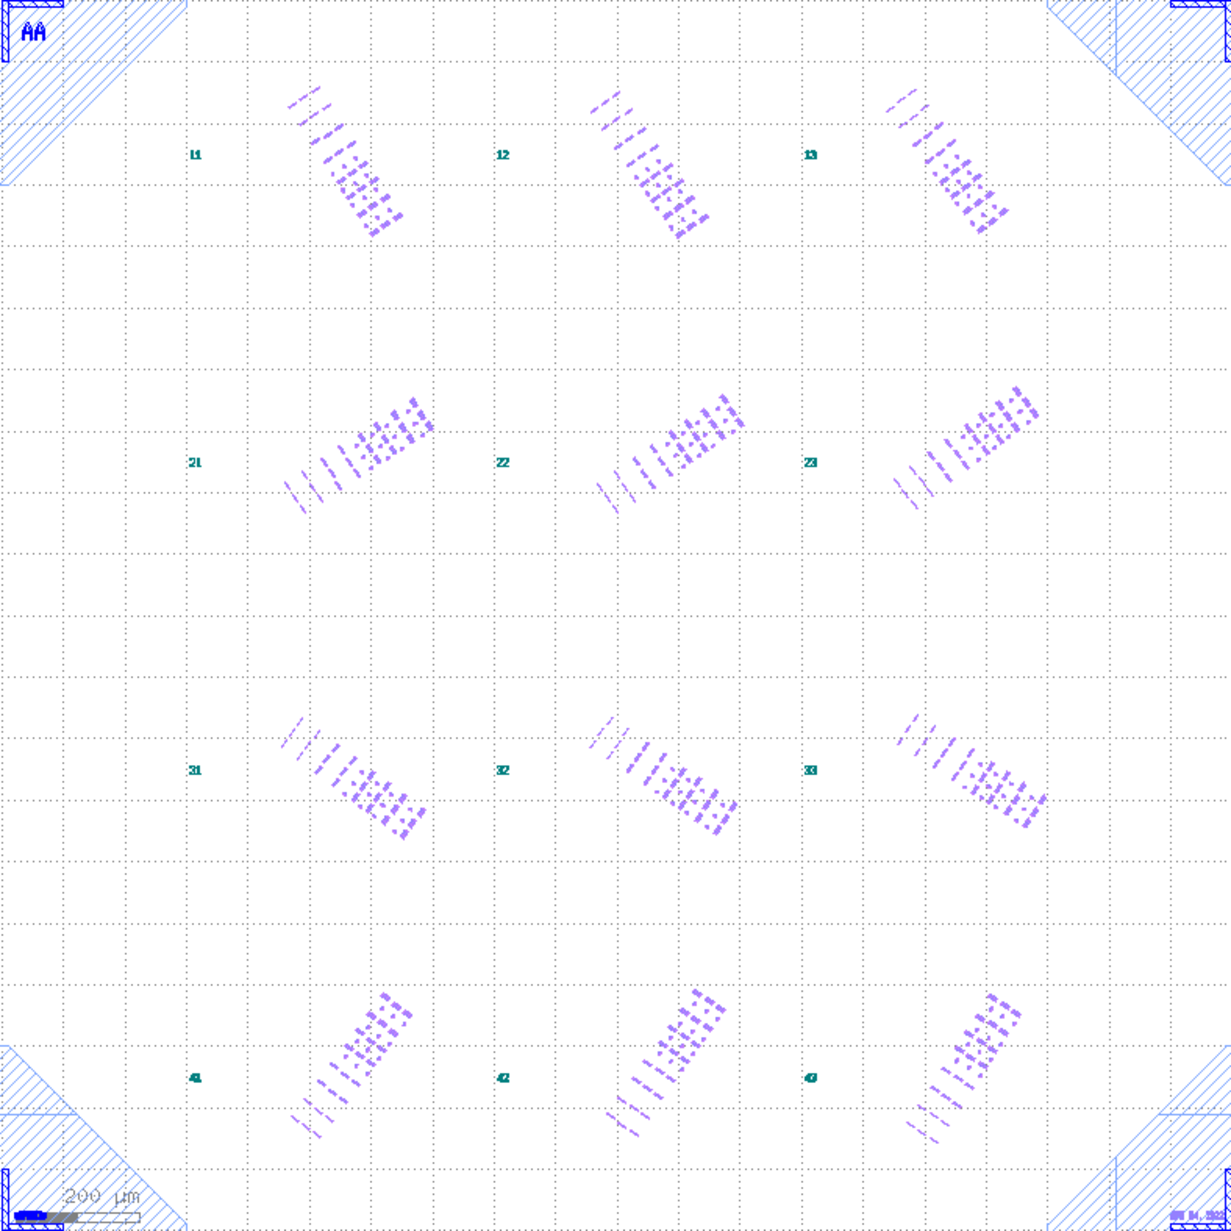
\includegraphics[width = 0.48\textwidth]{5_Yield_Analysis/Fig/mask_division.pdf}
    }
    \subcaptionbox{
        Mask of the chip.
        \label{subfig:mask_chip}
    }{
        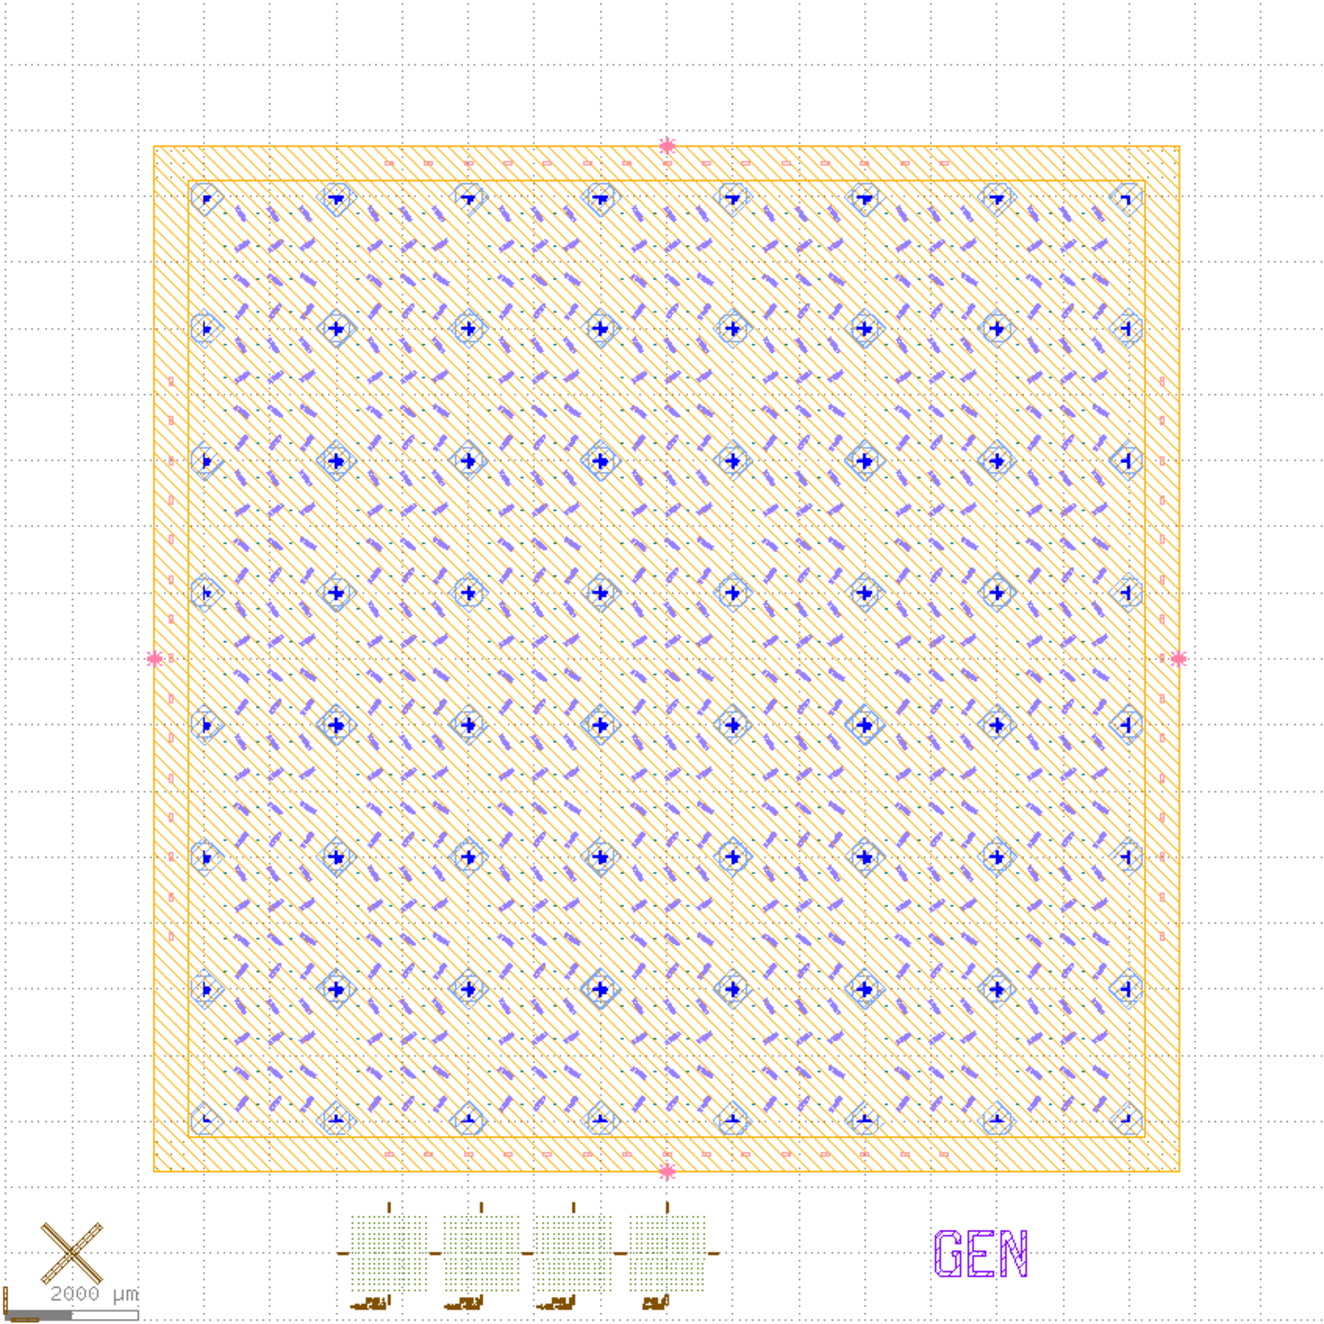
\includegraphics[width = 0.48\textwidth]{5_Yield_Analysis/Fig/mask_chip.pdf}
    }
    \caption[Mask used for the \acs{ebl} and optical lithography exposition of \hkl(1 1 0) substrtates.]{Mask used for the \acs{ebl} and optical lithography exposition of \hkl(1 1 0) substrates. The in-plane \hkl<1 1 0> direction runs parallel to the bottom margin of the images. \subref{subfig:mask_array} shows a single array of the kind illustrated in Figure~\ref{subfig:110_design2}. \subref{subfig:mask_section} shows a section of the chip, marked by the number 11, containing \num{24} arrays, \num{6} for each template width (\qty{70}{nm}, \qty{140}{nm}, \qty{210}{nm}, and \qty{280}{nm}). \num{12} merge structures are also visible. \subref{subfig:mask_division} shows a division of the chip, containing \num{12} sections. \subref{subfig:mask_chip} shows the full mask of the chip, containing \num{49} divisions. The sample area measuring \qtyproduct{1.5 x 1.5}{\centi\metre} is highlighted in yellow.}
    \label{fig:wafer_mask}
\end{figure}

The yield analysis will focus on samples \num{6} and \num{7}, grown on \hkl(1 1 0) \acs{soi} wafers, which were introduced in Sections~\ref{sec:s6} and \ref{sec:s7}, respectively. In particular, the yield calculations will involve single nucleation nanowires grown in arrays like those shown in Figure~\ref{subfig:110_design2}. These structures supported \num{66} nucleation sites each and were grown with 4 template widths: \qty{70}{nm}, \qty{140}{nm}, \qty{210}{nm}, and \qty{280}{nm}.

\subsection{Lithography masks}

Figure~\ref{fig:wafer_mask} shows the digital mask that was used during the \acs{tase} process in the \acf{ebl} definition of markers, micro-structures, and template openings and to fabricate the optical lithography mask used to create the marker protections, as explained in \ref{chap:tase}. Figure~\ref{subfig:mask_array} shows how a single \num{66}-nanowire array looks like in the \acs{ebl} mask. This single array is placed in a section, shown in Figure~\ref{subfig:mask_section}, of the chip, together with \num{23} others, totalling \num{6} array per nanowire size per section. Sections are further grouped in divisions, one of which, marked AA, is shown in Figure~\ref{subfig:mask_division}. Each division contains a total of \num{12} sections. Each of the sections is orientated so that the nanowires in each array and merge structure are closely aligned with one of the in-plane \hkl<1 1 1> directions, or \qty{20}{\degree} misaligned from them. This results in a series of fishbone patterns across the mask used to pattern the entire chip, shown in Figure~\ref{subfig:mask_chip}. The \qtyproduct{1.5 x 1.5}{\centi\metre} sample area of each chip, highlighted in yellow, contains \num{49} divisions, resulting in a total of \num{1254528} nanowire single nucleation sites (therefore, without taking into account the merge structures). 

Each section is identified by a number, in the case of the one in Figure~\ref{subfig:mask_section} it is \num{11}, and two letters that, in turn, identify the division of the mask in which it is found. Therefore, the naming convention defines, in order, the row and the column of the division within the chip, starting at the top left of Figure~\ref{subfig:mask_chip}, and the row and column of the section within the division, starting at the top left of each division. In this example, AA11 is the top-leftmost section in the entire chip.

A \acs{stem_m} analysis of every nanowire is impossible due to the damage caused by \acf{fib} lamella preparation to the area immediately surrounding each cut-out. Still, even if a single cut per array was performed, a total of \num{19008} lamellae would have to be manufactured and analysed per sample. This task is too time-consuming and resource-intensive to be viable. Therefore, a different approach must be found to tackle the problem of yield calculation.

\subsection{\texorpdfstring{Internal morphology and reproducibility in \acs{tase} nanowires}{Internal morphology and reproducibility in TASE nanowires}}

Stabilisation of a single \hkl{1 1 1} facet for the internal superlattice heterointerfaces of the nanowires was observed in all phosphide-arsenide samples since it was first achieved in sample 3 (Section~\ref{sec:s3}). Eliminating the ambiguity of facet selection due to the substrate \hkl(1 1 0) discussed in Section~\ref{sec:s4} limits the outcome of the \acf{tmah} etching to a single facet seed, a condition which is achieved reliably since sample 4. Similarly, from sample 4 onwards, the seed facet and the end facet of the wires have been parallel or showed a misalignment of \qty{3}{\degree} in sample 6 (Section~\ref{sec:s6}). Finally, with the minimisation of \acf{ingaas} nucleation layer thickness introduced in sample 5 (Section~\ref{sec:s5}) all important material layers are heterointerfaced with a single \hkl{1 1 1} facet.

\begin{figure}
    \centering
    \tikzsetnextfilename{s7_OVs}
    \begin{tikzpicture}
        \node[inner sep=0pt] (image) at (0,0) {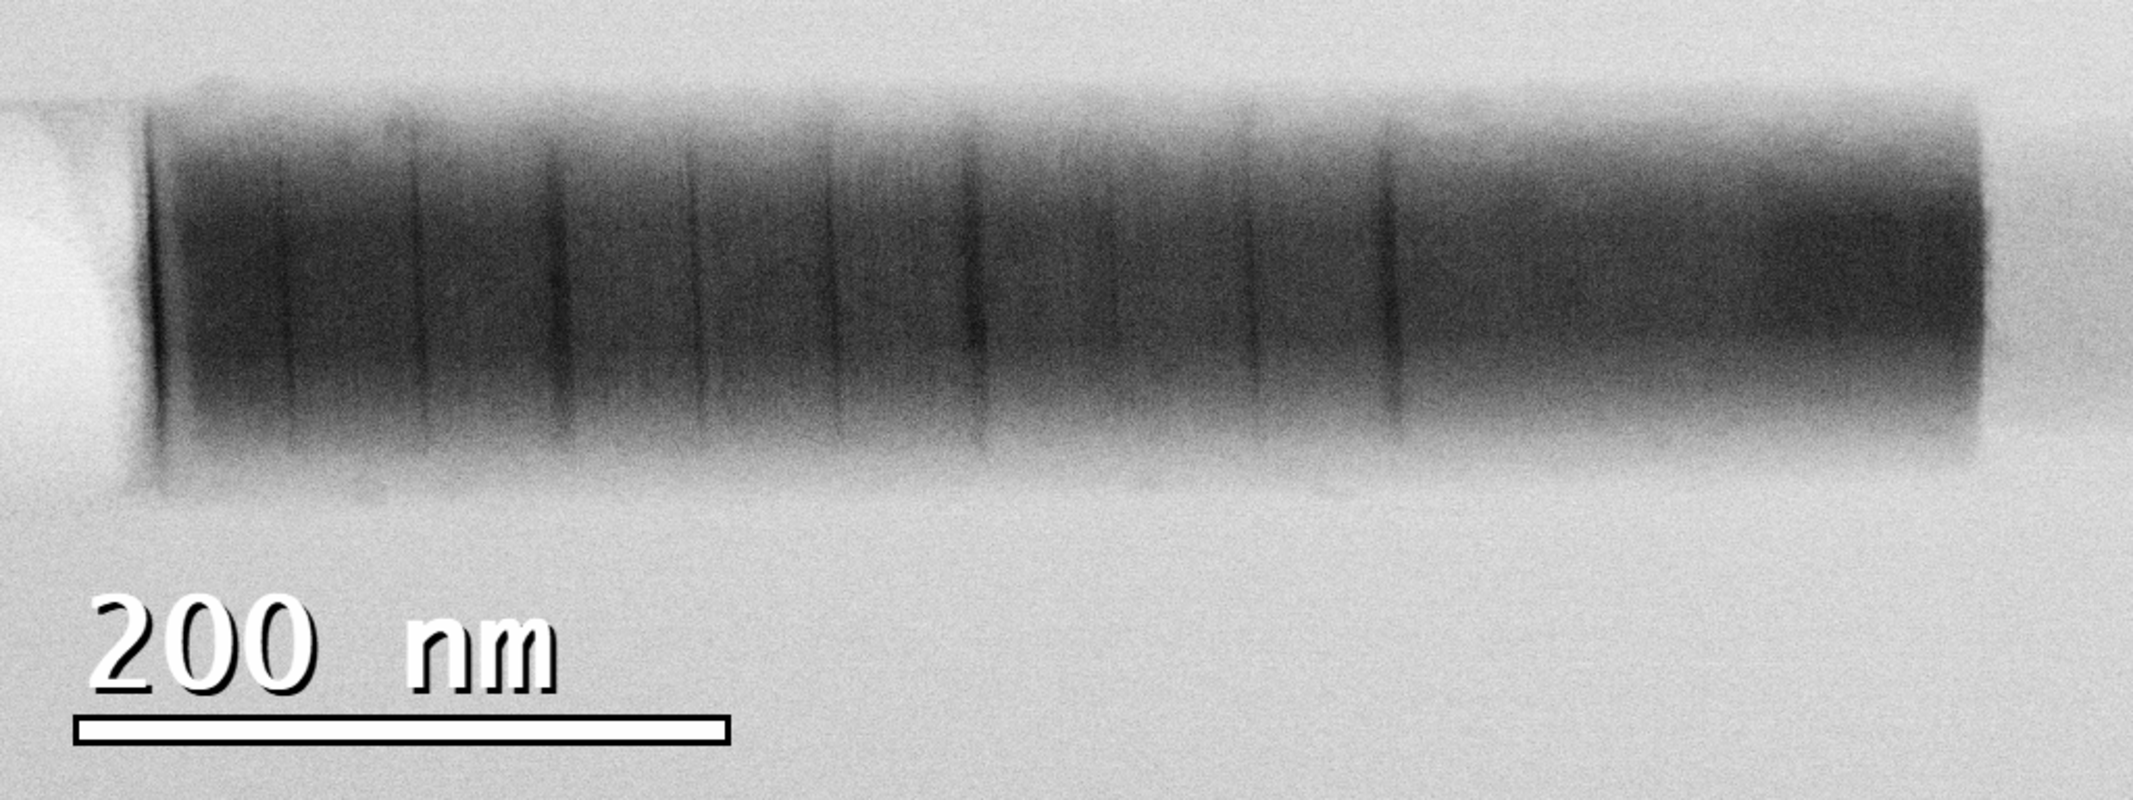
\includegraphics[width=0.48\textwidth]{5_Yield_Analysis/Fig/s7_OV1.pdf}};
        \node at (3,-0.8) {(1)};
        \node[inner sep=0pt] (image) at (8,0) {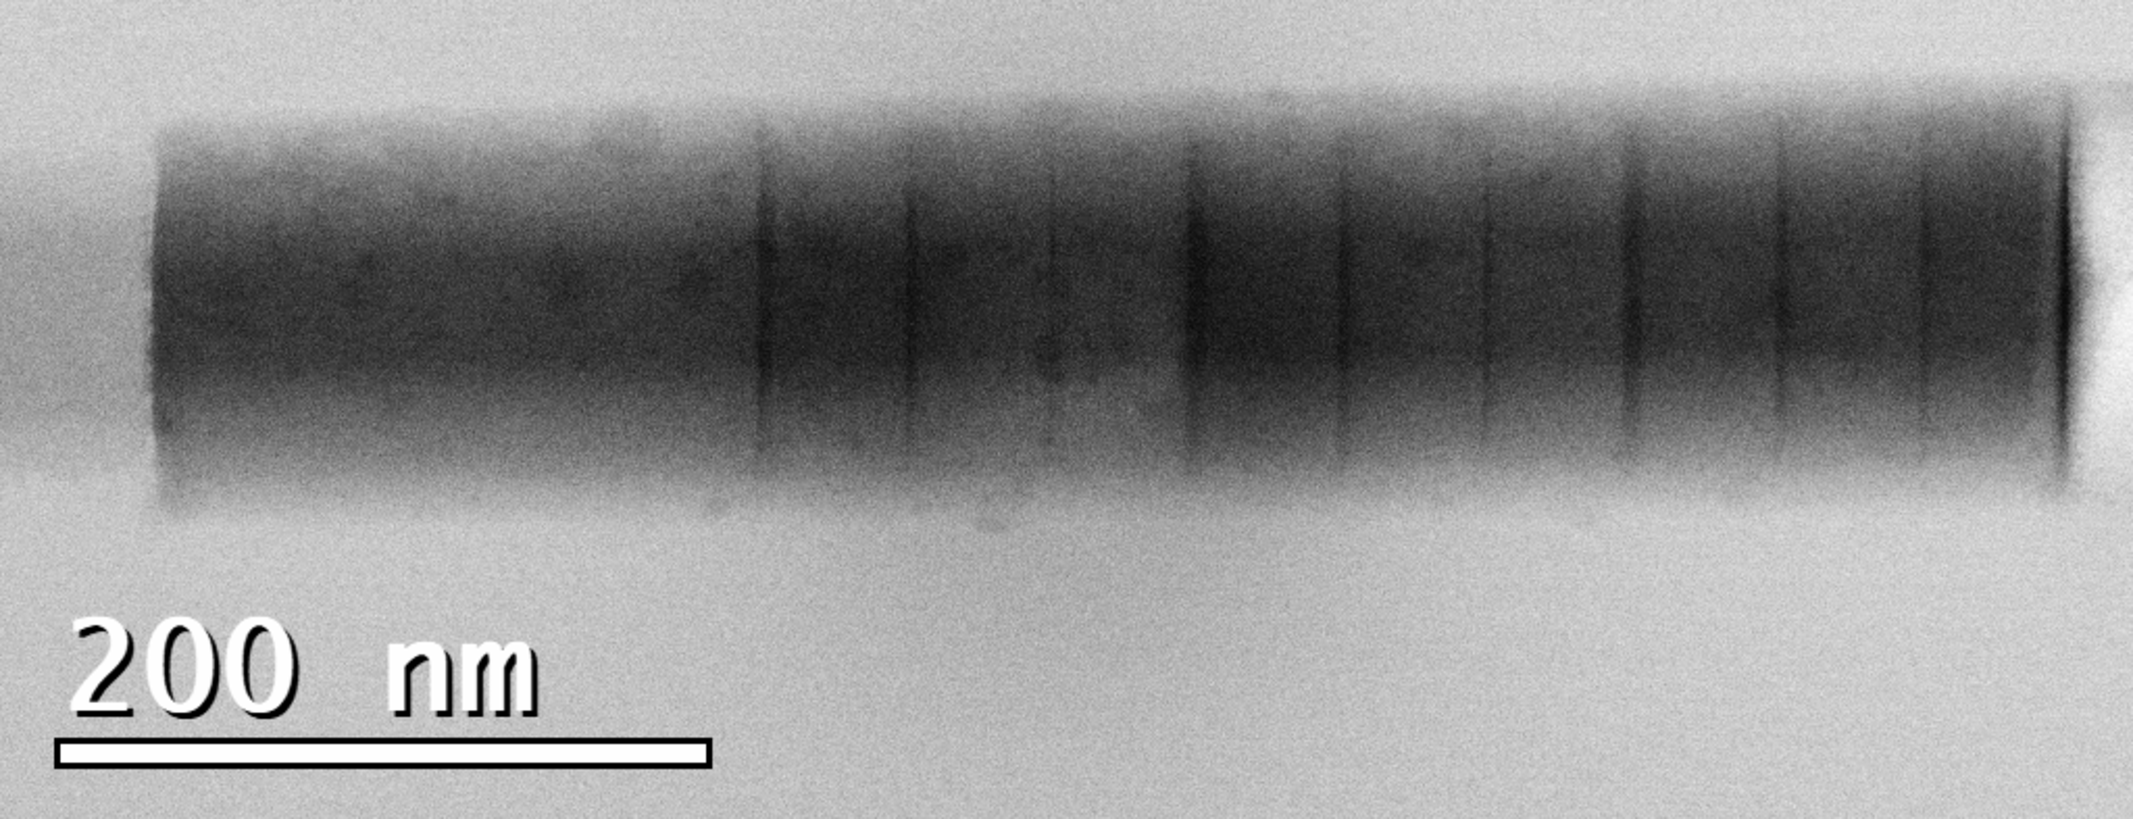
\includegraphics[width=0.48\textwidth]{5_Yield_Analysis/Fig/s7_OV2.pdf}};
        \node at (11,-0.8) {(2)};
        \node[inner sep=0pt] (image) at (0,-3) {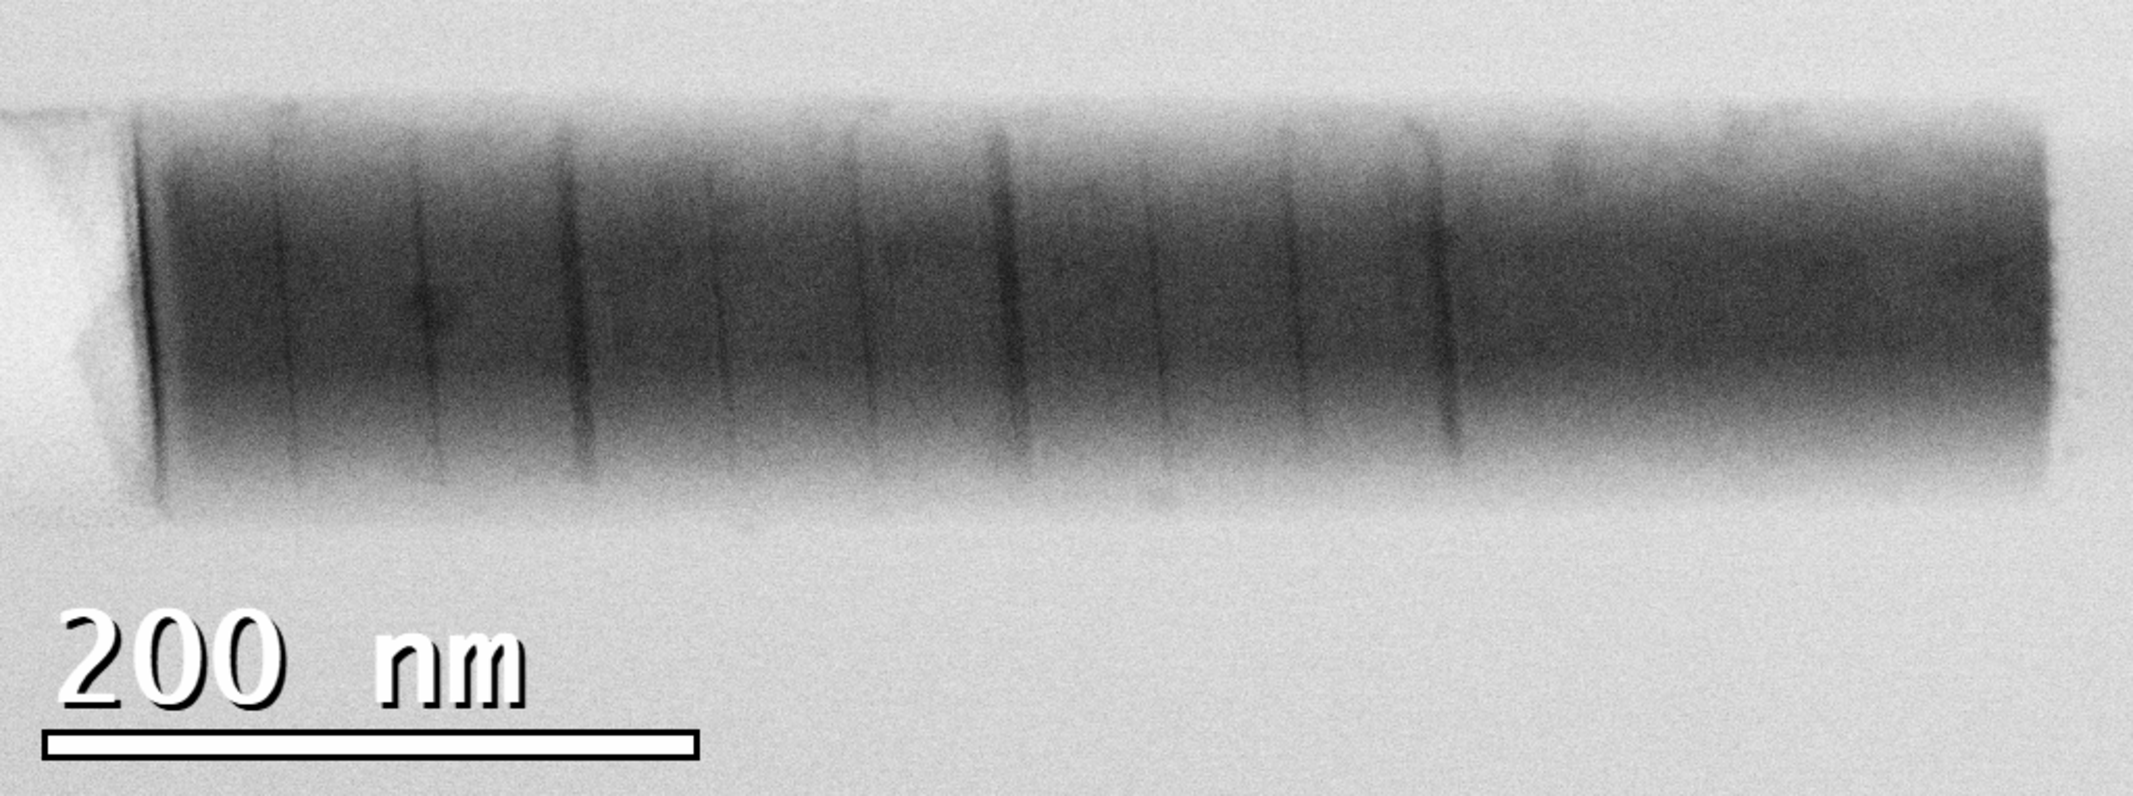
\includegraphics[width=0.48\textwidth]{5_Yield_Analysis/Fig/s7_OV3.pdf}};
        \node at (3,-3.8) {(3)};
        \node[inner sep=0pt] (image) at (8,-3) {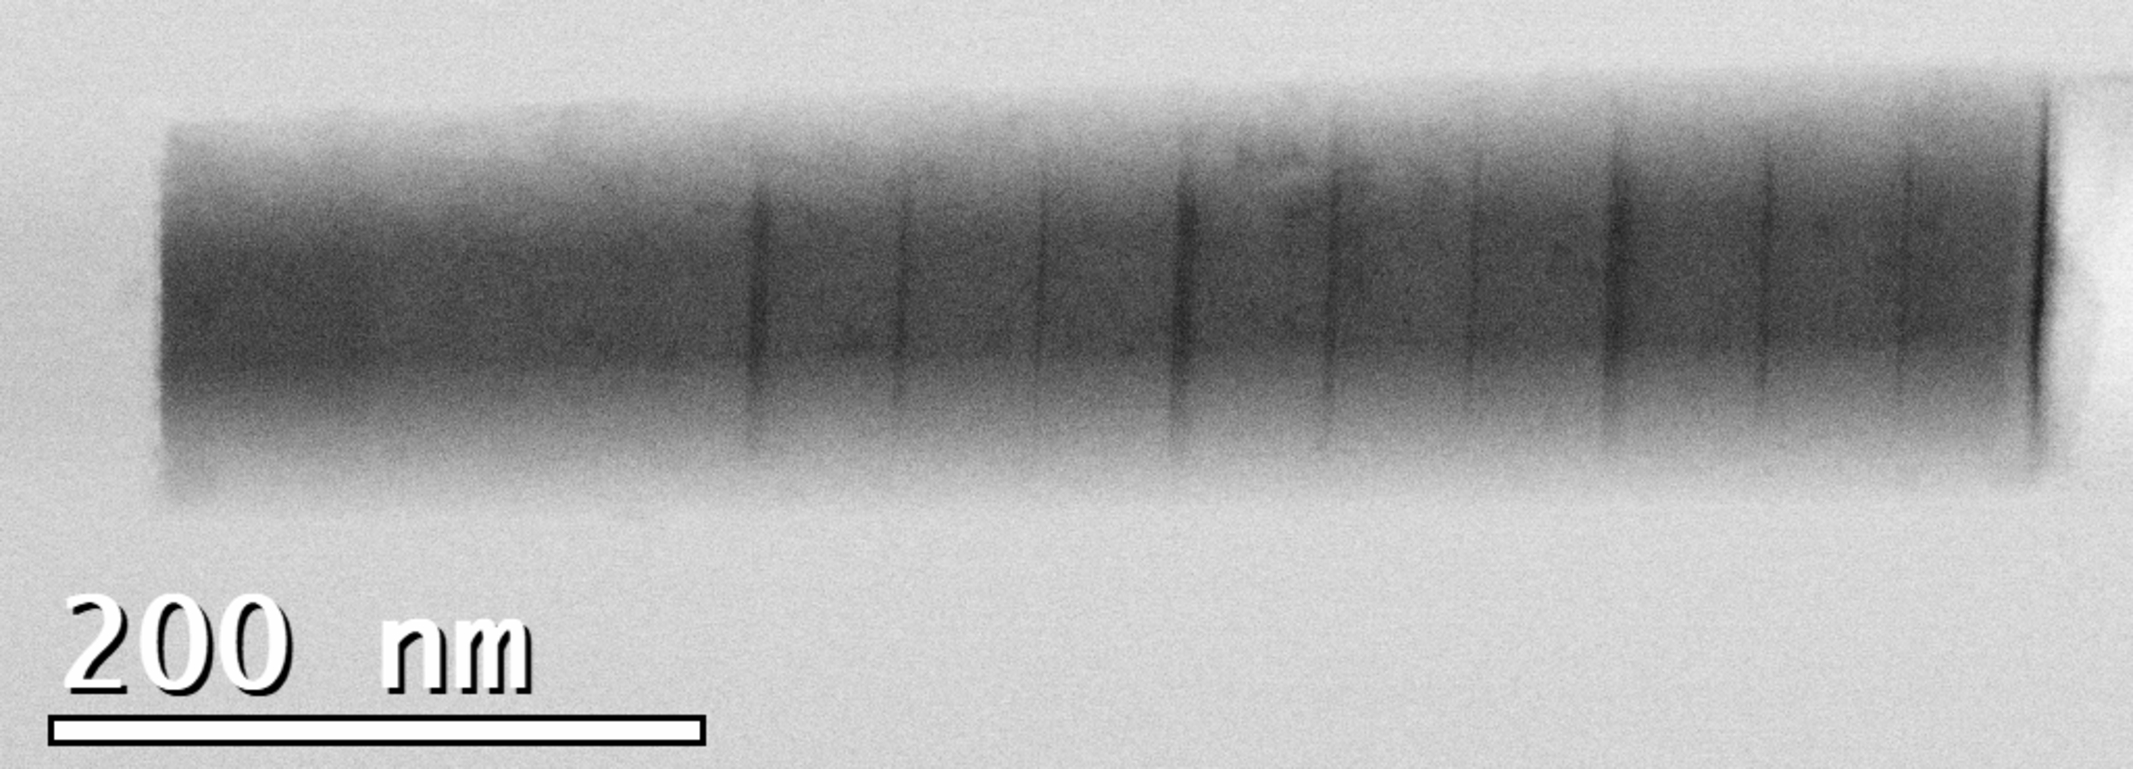
\includegraphics[width=0.48\textwidth]{5_Yield_Analysis/Fig/s7_OV4.pdf}};
        \node at (11,-3.8) {(4)};
    \end{tikzpicture}
    \caption[Four \acs{bf}-\acs{stem_m} images of different nanowires from the lamella cut for sample 7.]{Four \acs{bf}-\acs{stem_m} images of different nanowires from the lamella cut for sample 7.}
    \label{fig:s7_OVs}
\end{figure}

\begin{figure}
    \centering
    \subcaptionbox{
        \acs{sem_m} images of \qty{70}{\nano\metre}-wide nanowire arrays.
        \label{subfig:70nm_arrays}
    }{
        \tikzsetnextfilename{70nm_arrays}
        \begin{tikzpicture}
            \node at (0,1) {Perpendicular};
            \node[inner sep=0pt] (image) at (0,0) {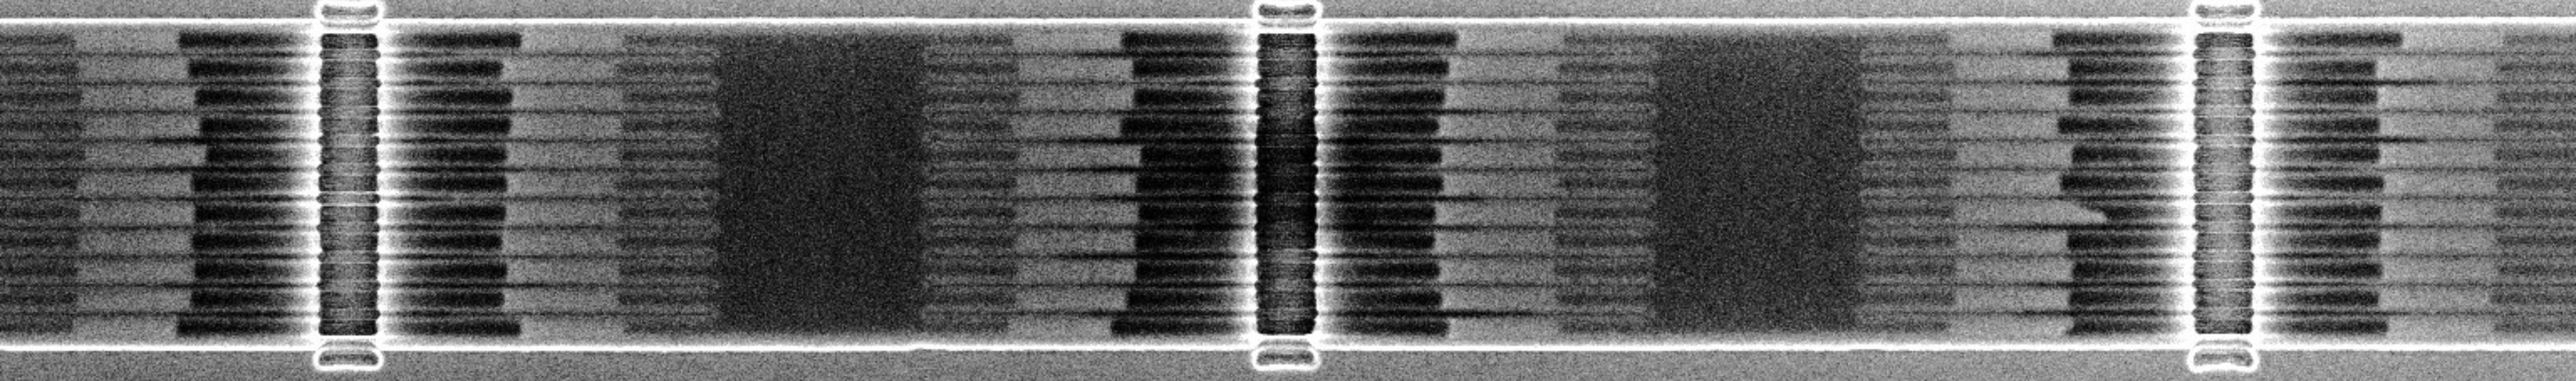
\includegraphics[width=0.48\textwidth]{5_Yield_Analysis/Fig/70nm_perpendicular.pdf}};
            \draw[yellow, -stealth] (1.2, -0.06) -- ++ (0.5, 0);
            \node at (8,1) {\qty{20}{\degree} misaligned};
            \node[inner sep=0pt] (image) at (8,0) {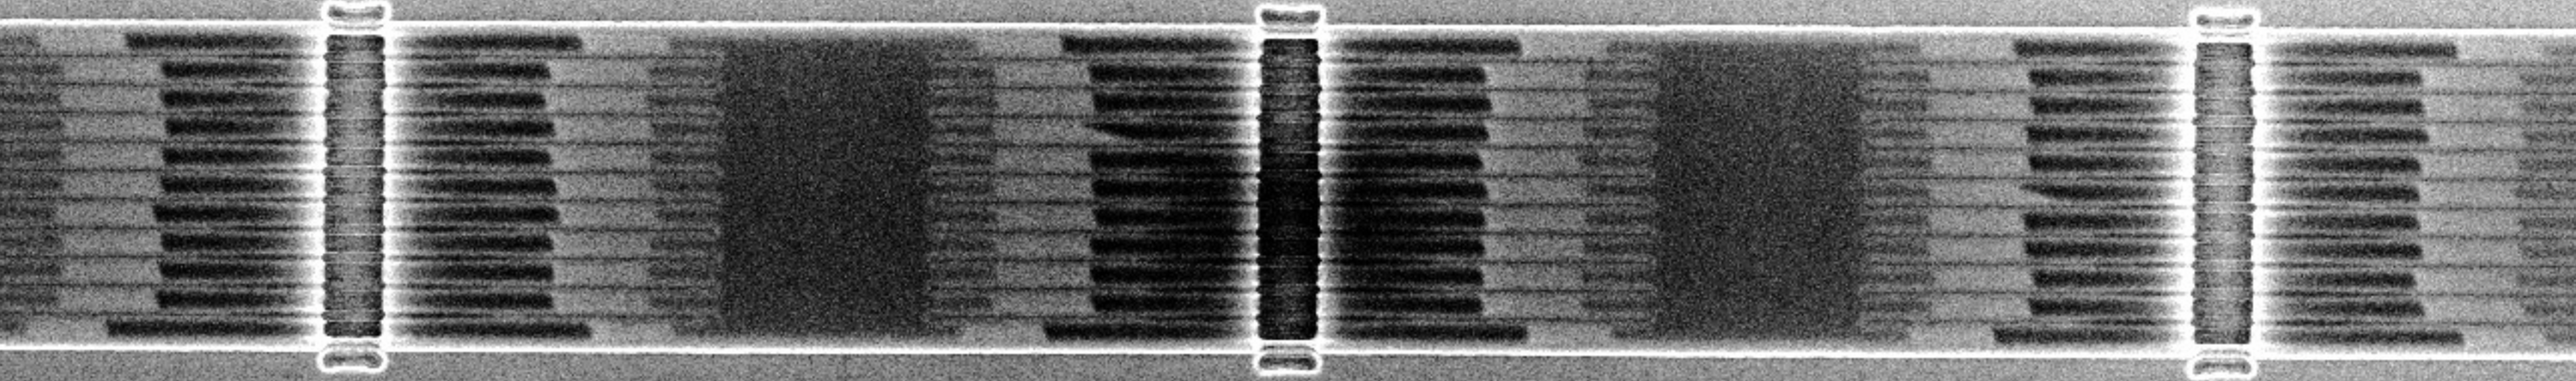
\includegraphics[width=0.48\textwidth]{5_Yield_Analysis/Fig/70nm_misaligned.pdf}};
            \draw[yellow, -stealth] (6.5, 0.18) -- ++ (0.5, 0);
            \draw[yellow, -stealth] (9.2, 0) -- ++ (0.5, 0);
            \draw[| - |] (2.4, -0.9) -- ++ (3.2, 0) node [anchor = west] {\qty{5}{\micro\metre}};
        \end{tikzpicture}
    }
    \subcaptionbox{
        \acs{sem_m} images of \qty{140}{\nano\metre}-wide nanowire arrays. Scale bar in \subref{subfig:280nm_arrays}.
        \label{subfig:140nm_arrays}
    }{
        \tikzsetnextfilename{140nm_arrays}
        \begin{tikzpicture}
            \node[inner sep=0pt] (image) at (0,0) {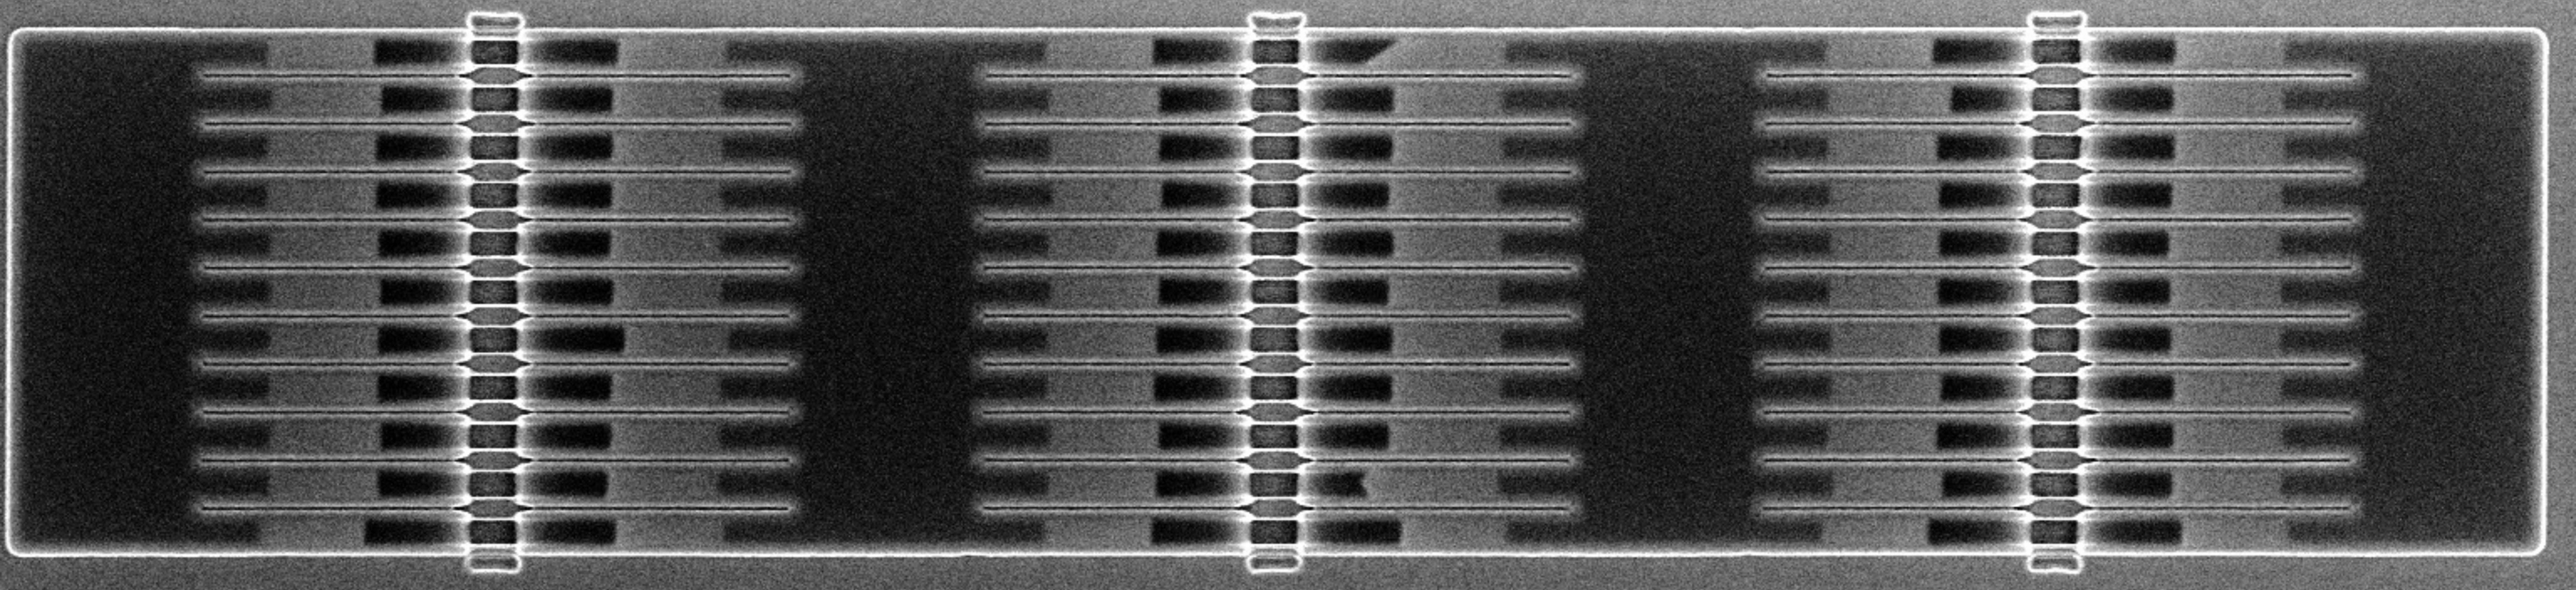
\includegraphics[width=0.48\textwidth]{5_Yield_Analysis/Fig/140nm_perpendicular.pdf}};
            \draw[yellow, -stealth] (1.4, 0.73) -- ++ (-0.5, 0);
            \draw[yellow, -stealth] (1.4, -0.56) -- ++ (-0.5, 0);
            \node[inner sep=0pt] (image) at (8,0) {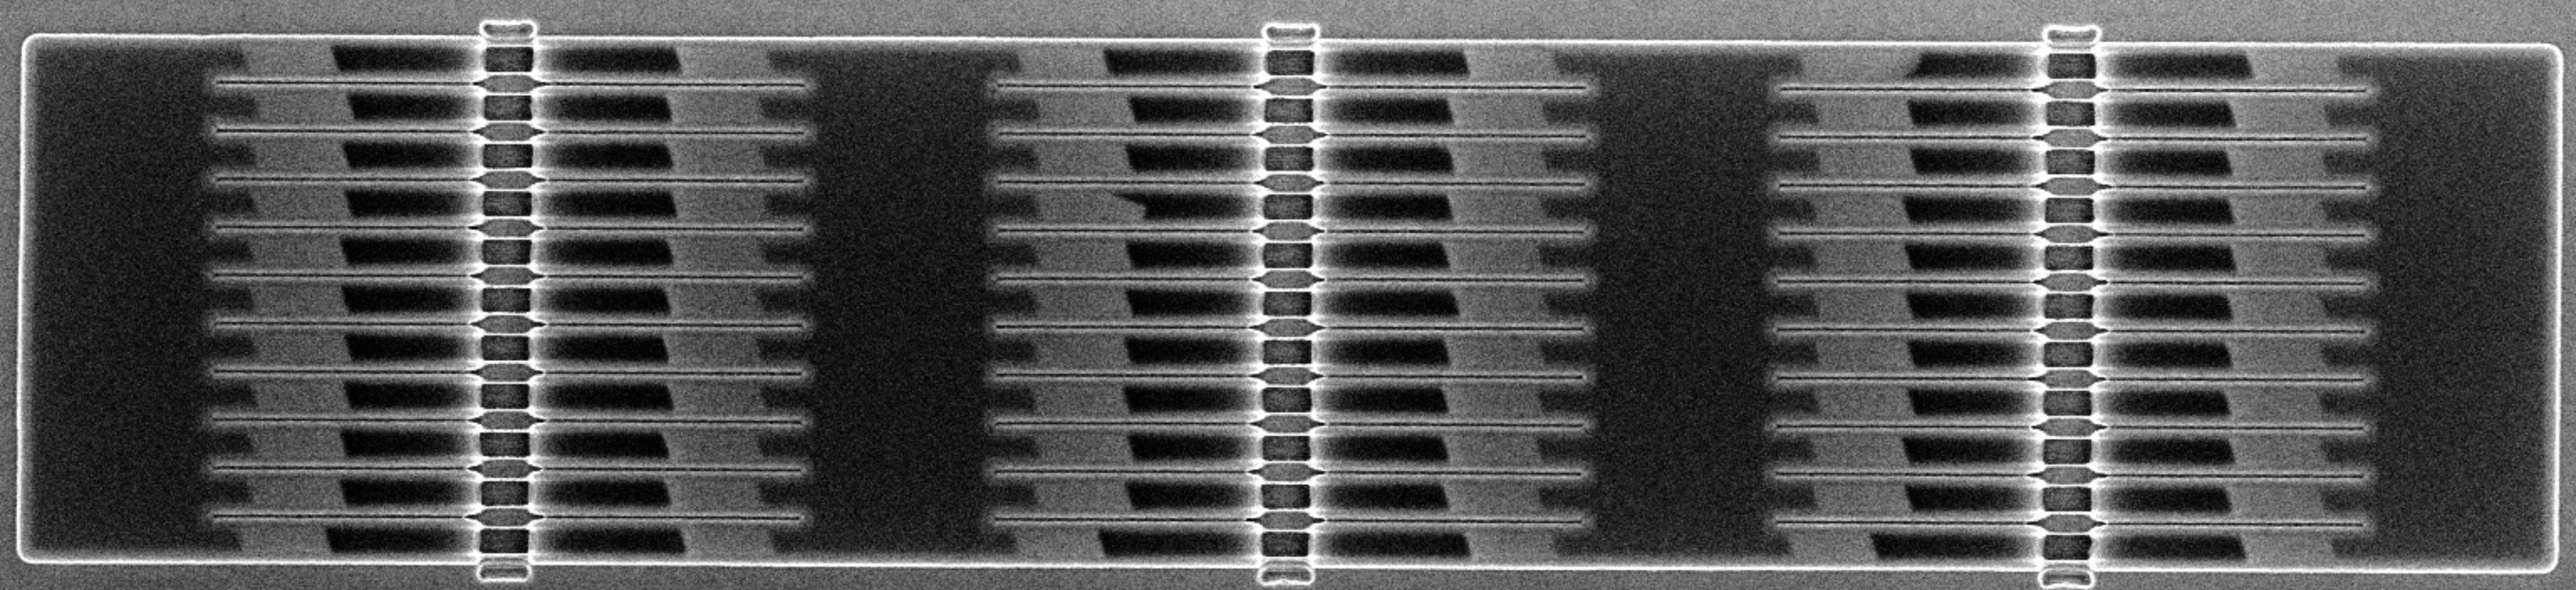
\includegraphics[width=0.48\textwidth]{5_Yield_Analysis/Fig/140nm_misaligned.pdf}};
            \draw[yellow, -stealth] (6.6, 0.27) -- ++ (0.5, 0);
        \end{tikzpicture}
    }
    \subcaptionbox{
        \acs{sem_m} images of \qty{210}{\nano\metre}-wide nanowire arrays. Scale bar in \subref{subfig:280nm_arrays}.
        \label{subfig:210nm_arrays}
    }{
        \tikzsetnextfilename{210nm_arrays}
        \begin{tikzpicture}
            \node[inner sep=0pt] (image) at (0,0) {\includegraphics[width=0.48\textwidth]{5_Yield_Analysis/Fig/210nm_perpendicular.pdf}};
            \node[inner sep=0pt] (image) at (8,0) {\includegraphics[width=0.48\textwidth]{5_Yield_Analysis/Fig/210nm_misaligned.pdf}};
            \draw[yellow, -stealth] (7, -0.87) -- ++ (-0.5, 0);
        \end{tikzpicture}
    }
    \subcaptionbox{
        \acs{sem_m} images of \qty{280}{\nano\metre}-wide nanowire arrays.
        \label{subfig:280nm_arrays}
    }{
        \tikzsetnextfilename{280nm_arrays}
        \begin{tikzpicture}
            \node[inner sep=0pt] (image) at (0,0) {\includegraphics[width=0.48\textwidth]{5_Yield_Analysis/Fig/280nm_perpendicular.pdf}};
            \draw[yellow, -stealth] (1.4, 0.3) -- ++ (-0.5, 0);
            \node[inner sep=0pt] (image) at (8,0) {\includegraphics[width=0.48\textwidth]{5_Yield_Analysis/Fig/280nm_misaligned.pdf}};
            \draw[yellow, -stealth] (4.3, 1.45) -- ++ (0.5, 0);
            \draw[yellow, -stealth] (11.7, 0.25) -- ++ (-0.5, 0);
            \draw[yellow, -stealth] (11.7, -0.05) -- ++ (-0.5, 0);
            \draw[| - |] (2.6, -2) -- ++ (2.7, 0) node [anchor = west] {\qty{5}{\micro\metre}};
        \end{tikzpicture}
    }
    \caption[\acs{sem_m} images of nanowire arrays.]{\acs{sem_m} top-view images of III-V nanowire arrays with defective wires marked by yellow arrows. \subref{subfig:70nm_arrays}, \subref{subfig:140nm_arrays}, \subref{subfig:210nm_arrays}, and \subref{subfig:280nm_arrays} show both perpendicular and \qty{20}{\degree} misalligned arrays with template widths of \qty{70}{nm}, \qty{140}{nm}, \qty{210}{nm}, and \qty{280}{nm}, respectively \cite{Brugnolotto2023_2}.}
    \label{fig:s7_arrays}
\end{figure}

Figure~\ref{fig:s7_OVs} shows four \acs{bf}-\acs{stem_m} overview images of the same number of nanowires from the lamella cut from sample 7. These images confirm the observations made in the previous paragraph regarding the relation between \acf{si} / III-V semiconductor interface and the nanowire end-facet shapes mirrored in all important interior phosphide-arsenide heterointerfaces. An approximation can therefore be made by inferring that if the \acl{si} seed consists of a single \hkl{1 1 1} facet, the III-V material fully covers it, and the end-wire surface is a single \hkl{1 1 1} facet parallel to the \acs{si} seed the internal morphology also developed as-desired, with \hkl{1 1 1} single-facet heterointerfaces. Therefore, these metrics can be used to define a perfect wire.

These specifications do not require a full \acs{stem_m} analysis. Instead, a \acs{sem_m} survey of the arrays in the sample is sufficient to assess the growth yield. One such survey, resulting in an open access dataset \cite{dataset}, was carried out on samples 6 and 7. Figure~\ref{fig:s7_arrays} shows eight images of the arrays of sample 6 taken from this dataset. A first distinction can be made by "Perpendicular" wires, so-called because the heterointerfaces in perfect nanowires are perpendicular to all four template walls, and \qty{20}{\degree} misaligned wires, which owe their name to the tilt of the template channels from the \hkl{1 1 1} direction.

The dataset was collected manually using the \acs{sem_m} beam of the dual-beam \acs{sem_m} - \acs{fib} tool. Due to project time constraints, sampling became necessary to gather a full suite of images representative of the \num{19008} arrays. Five sections were selected in each chip, mostly at random. However, for sample 7, a perpendicular and a \qty{20}{\degree} misaligned section in the AA division were selected to ensure a representation of the border divisions of the chip. Another difference between the two samples is that while for sample 6, sections were randomly drafted and changed for each of the five positions, for sample 6, a second division was randomly selected, within which two more sections were imaged. The fifth and final section was once again randomly chosen. These sections are reported in Table~\ref{tab:dataset_sections}. Three parallel and two \qty{20}{\degree} misaligned sections were imaged for both samples.

\begin{table}
    \centering
    \caption{Randomly selected sections for the array dataset.}
    \begin{tabular}{c|c c c c c}
         & \multicolumn{5}{c}{Sections} \\ \hline
        Sample 6 & BB13 & CD22 & DE42 & FB13 & GG31 \\
        Sample 7 & AA32 & AA41 & DE11 & DE22 & FC11 \\ \hline \hline
    \end{tabular}
    \label{tab:dataset_sections}
\end{table}

This means that 240 arrays containing 15840 nucleation sites were imaged. This number represents \qty{0.63}{\percent} of the wires in the two chips. As such, it can be helpful to provide a first estimate of the yield, and for a dataset from which automated yield calculation methods can be built on.

\subsection{\texorpdfstring{\acs{sem_m}-observable defects in \acs{tase} nanowires}{SEM observable defects in TASE nanowires}}

\begin{figure}
    \centering
    \subcaptionbox{
        Parasitic growth covering some growth sites in sample 7.
        \label{subfig:defects_parasitic}
    }{
        \tikzsetnextfilename{defects_parasitic}
        \begin{tikzpicture}
            \node[inner sep=0pt] (image) at (0,0) {\includegraphics[width=\textwidth]{5_Yield_Analysis/Fig/defects_parasitic.pdf}};
            \draw[| - |] (-2.7, -3) -- ++ (5.5, 0) node [anchor = west] {\qty{5}{\micro\metre}};
        \end{tikzpicture}
    }
    \subcaptionbox{
        Un-nucleated sites in sample 7.
        \label{subfig:defects_unucleated}
    }{
        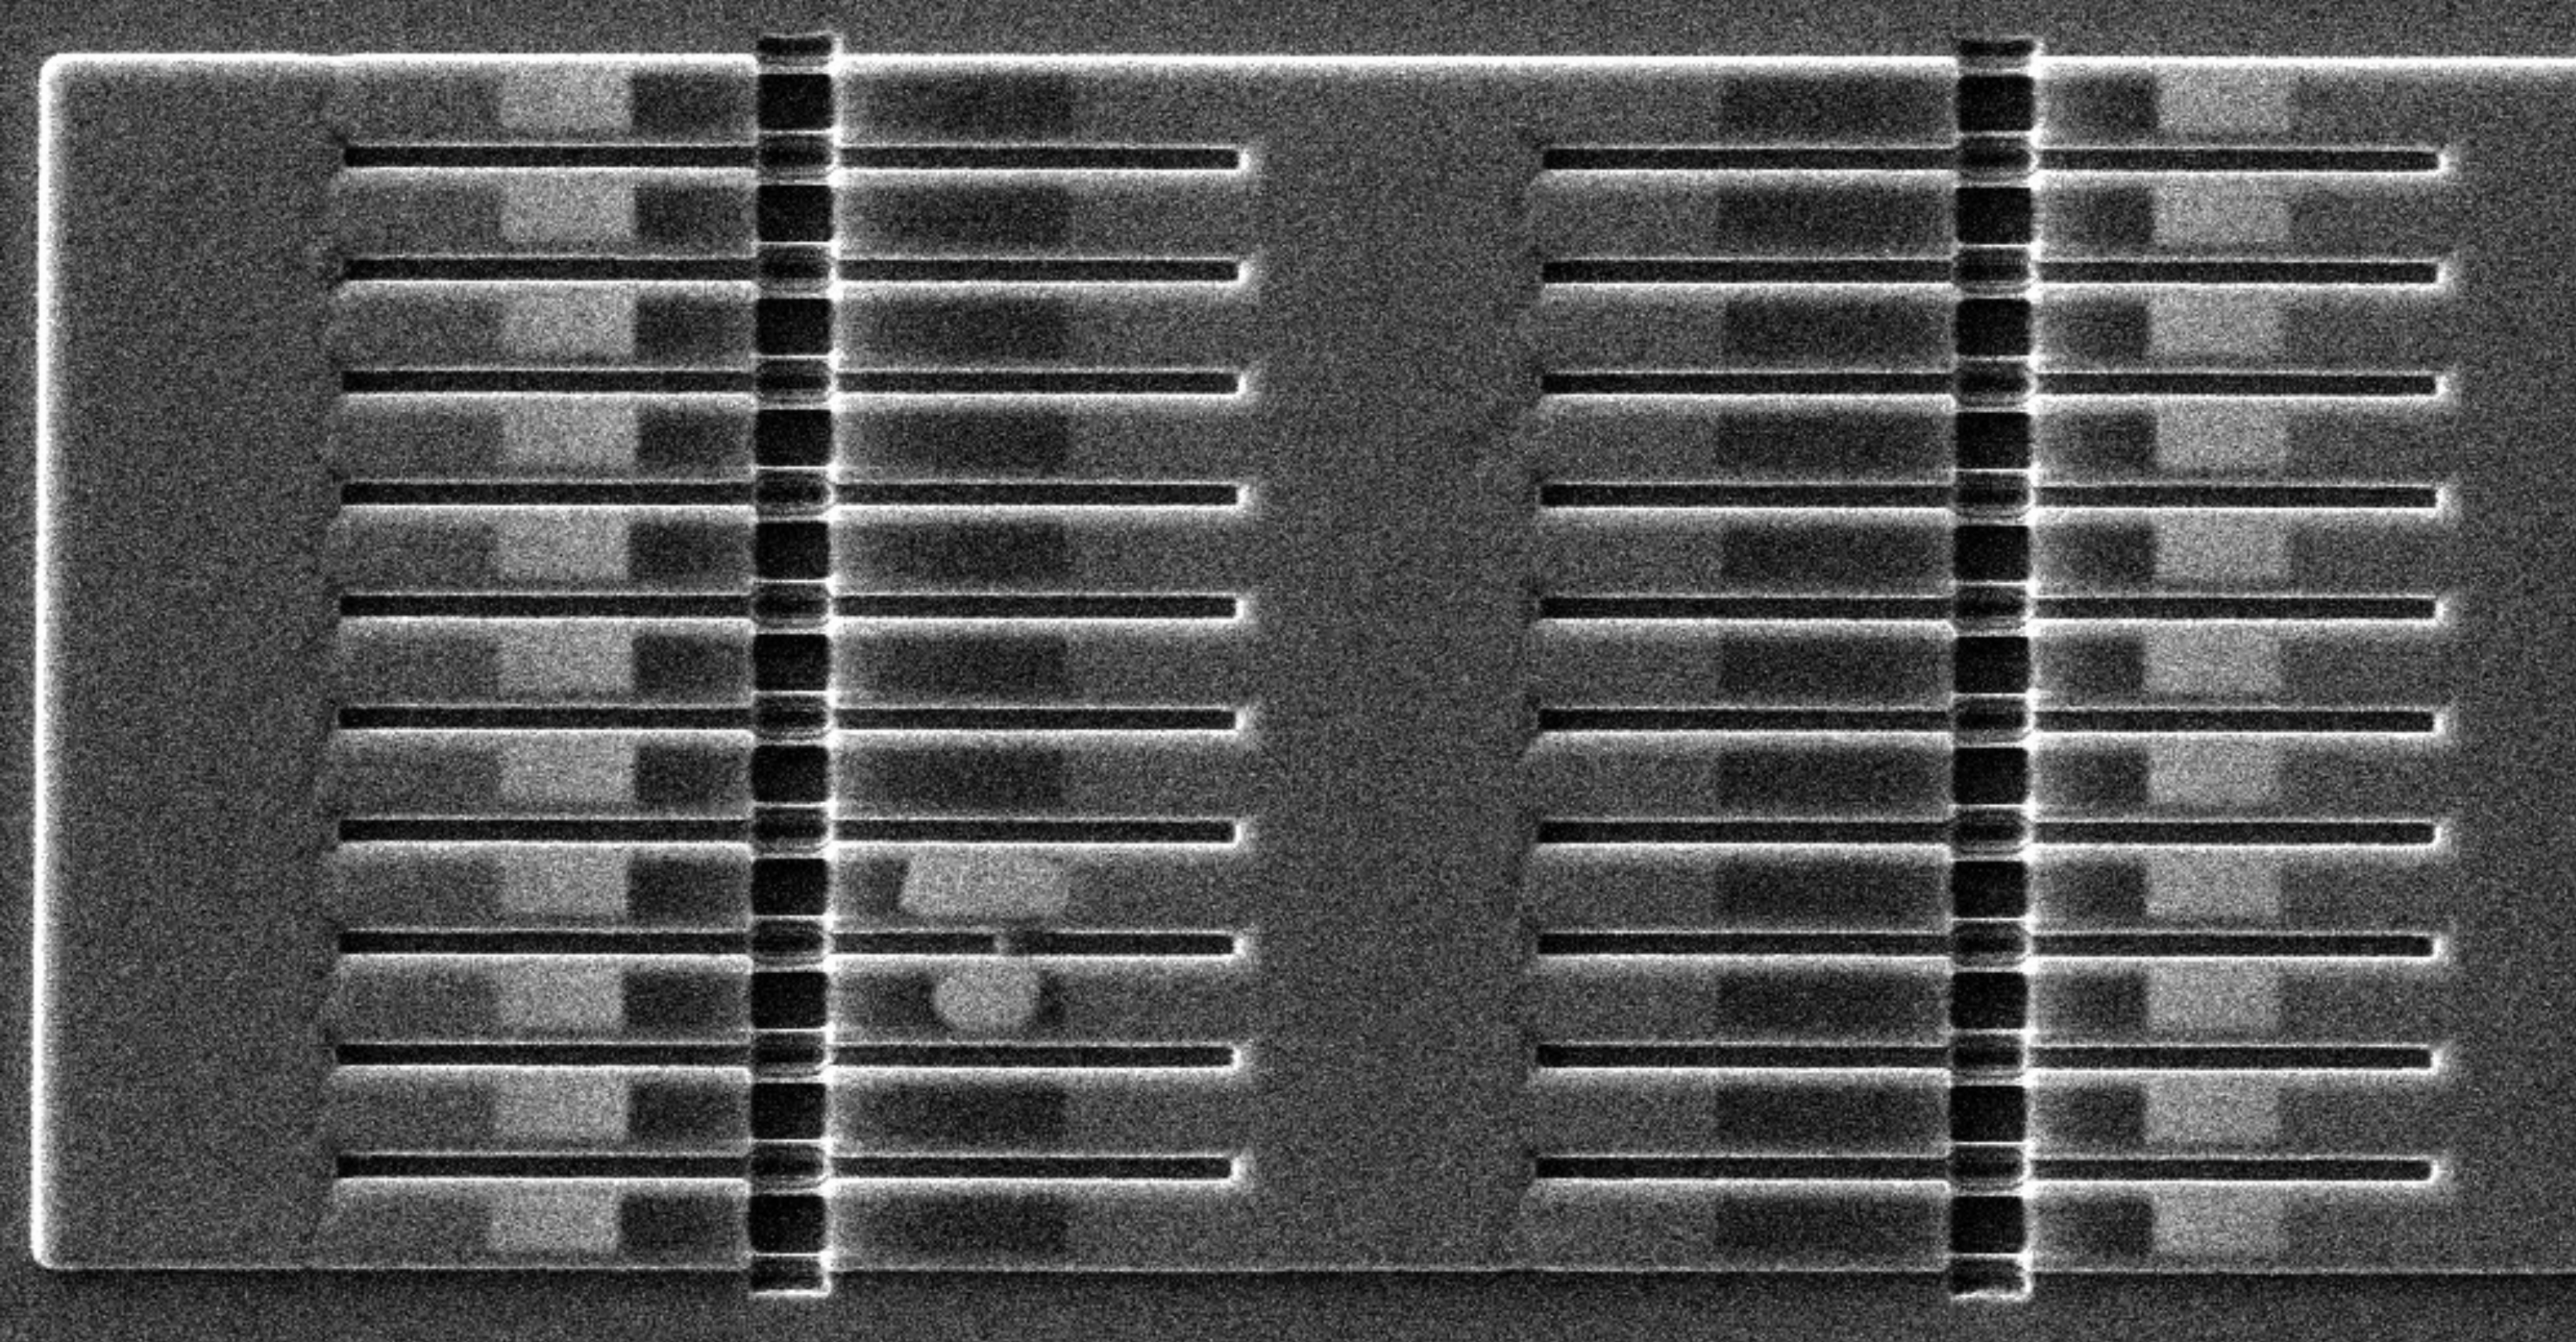
\includegraphics[width=0.665\textwidth]{5_Yield_Analysis/Fig/defects_unucleated.pdf}
    }
    \subcaptionbox{
        Template nucleation.
        \label{subfig:defects_oxide_nucleated}
    }{
        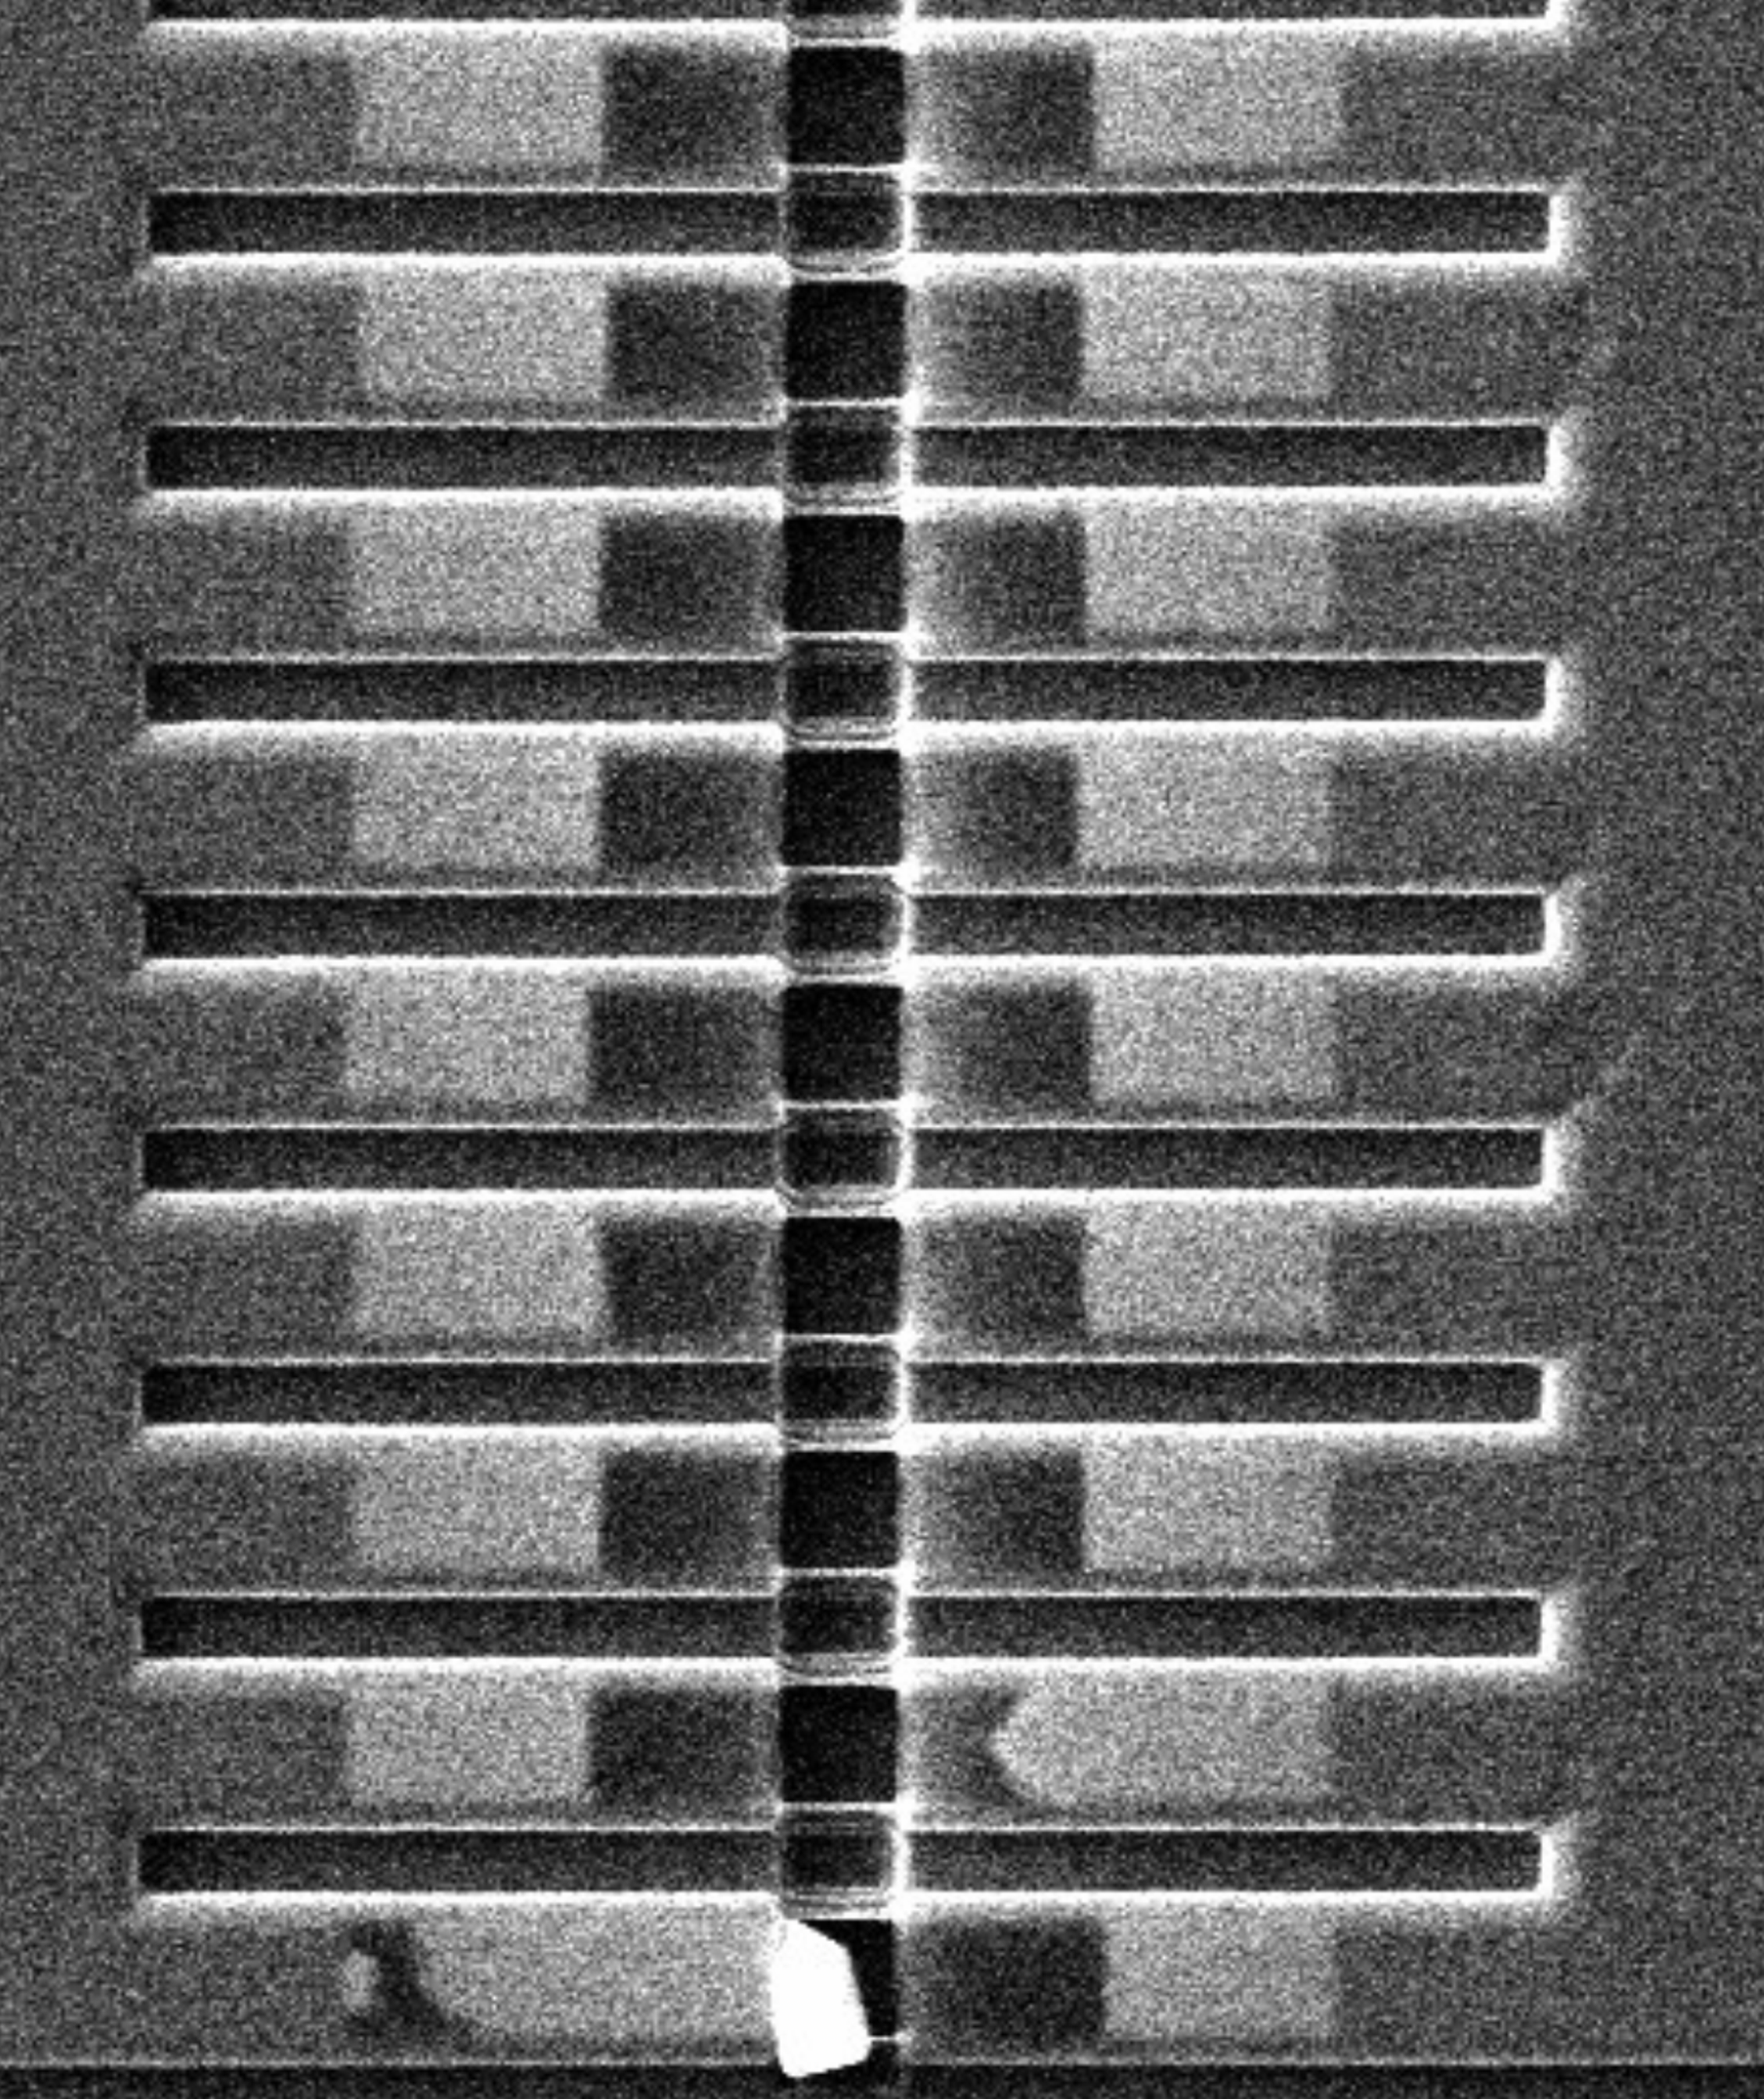
\includegraphics[width=0.29\textwidth]{5_Yield_Analysis/Fig/defects_oxide_nucleated.pdf}
    }
    \caption[Arrays from sample 7 presenting different types of defects.]{Arrays from sample 7 presenting different types of defects. The scale bar for all three images is in \subref{subfig:defects_parasitic}. \subref{subfig:defects_parasitic} shows a parasitic crystal hiding numerous nucleation sites from view. \subref{subfig:defects_unucleated} shows several nucleation sites where nucleation has not occurred. Two sites also contain defective wires. \subref{subfig:defects_oxide_nucleated} shows a template with nucleation on the \acs{si} seed, resulting in a small III-V particle, while the larger wire nucleated on the \acs{sio2} wall and grew out of the template.}
    \label{fig:defects}
\end{figure}

Defective wires were marked with yellow arrows in the nanowire arrays of Figure~\ref{fig:s7_arrays}. All these defective wires can be detected by looking at the wire-end interface. None of the wires mirroring the defective wires are defective, except for two. Each defective wire is isolated, having no immediate defective neighbour. Some of the defective wires also have partially covered seeds, as is most evident in the two neighbouring \qty{280}{\nano\metre} \qty{20}{\degree} misaligned array. However, unideal nucleation is not the only reason for defective growth, as seen in the \qty{140}{\nano\metre} and \qty{280}{\nano\metre} perpendicular wires, which fully cover the \acl{si} seed.

The length of the nanowires does not change significantly with the change in width of the \acs{tase} templates, as can be seen by comparing the lengths of the nanowires in Figure~\ref{subfig:70nm_arrays} with those of the nanowires in Figure~\ref{subfig:140nm_arrays}, \ref{subfig:210nm_arrays}, and \ref{subfig:280nm_arrays}, once the slight magnification used for presentation purposes in Figure~\ref{subfig:70nm_arrays} is taken into account. Therefore, compared to their neighbours, abnormally long or short III-V material segments in some nucleation sites can indicate undesired defects in the wire's internal structure.

Loss of growth selectivity can negatively affect the yield of "perfect" nanowires. In Figure~\ref{subfig:defects_parasitic}, the large parasitic crystal in the centre of the image hides many nucleation sites from view. Parasitic crystals often grow in places where impurities or geometric features on the surface of the chip provide unwanted nucleation sites. The lack of nucleation at several growth sites shown in Figure~\ref{subfig:defects_unucleated} can be considered another "defect" because it does not produce a nanowire where one is expected. Lack of nucleation occurs when a \acs{sio2} layer covers the \acl{si} seed and, therefore, is caused by \acf{hf} not entirely stripping this passivating layer or being unable to reach it due, for example, to the presence of a bubble on the chip surface during the pre-growth \acs{hf} dip. In Figure~\ref{subfig:defects_unucleated}, this defect occurs in nucleation sites that share their template opening with "perfect" nanowires, making the bubble hypothesis less likely. Figure~\ref{subfig:defects_oxide_nucleated} shows a growth site where nucleation co-occurred on both the \acl{si} seed surface and the \acs{sio2} inner template wall. The crystal nucleated on the \acl{si} surface was quickly cut off from the precursor supply when the other crystal grew to fill the width of the template. The defective crystal then grew faster than the other crystals around it due to its starting point being closer to the template opening and the random crystalline orientation resulting from the nucleation on the template wall. Had the undesired nucleation occurred closer to the opening of the template, it could have resulted in a parasitic growth similar to that in Figure~\ref{subfig:defects_parasitic}.

\section{Yield study}

\sisetup{detect-all = true}
\begin{table}
    \centering
    \caption[Overview of the distribution of defect types for samples 6 and 7.]{Overview of the distribution of defect types for samples 6 and 7 \cite{Brugnolotto2023_2}.}
    \begin{tabular}{l|ccccccc}
        \hline
         & \multicolumn{7}{c}{Defect categories and occurrence} \\ 
         & $\begin{matrix} \text{Wrong} \\ \text{Facet} \end{matrix}$ & $\begin{matrix} \text{Hidden by} \\ \text{Parasitic} \end{matrix}$ & $\begin{matrix} \text{Oxide} \\ \text{Nucleated} \end{matrix}$ & $\begin{matrix} \text{Seed} \\ \text{Exposed} \end{matrix}$ & Long & Short & Ungrown \\ 
        \hline \hline
        Sample 6 & \num{164} & \num{230} & \num{2} & \num{0} & \num{5} & \num{204} & \num{61} \\ 
        \textit{\% of category} & \textit{\qty{44.6}{\%}} & \textit{\qty{47.2}{\%}} & \textit{\qty{11.8}{\%}} & \textit{\qty{0}{\percent}} & \textit{\qty{62.5}{\%}} & \textit{\qty{98.8}{\%}} & \textit{\qty{75.3}{\%}} \\ 
        \hline
        Sample 7 & \num{204} & \num{257} & \num{15} & \num{8} & \num{3} & \num{7} & \num{20} \\ 
        \textit{\% of category} & \textit{\qty{55.4}{\%}} & \textit{\qty{52.8}{\%}} & \textit{\qty{88.2}{\%}} & \textit{\qty{100}{\%}} & \textit{\qty{37.5}{\%}} & \textit{\qty{1.2}{\%}} & \textit{\qty{24,7}{\%}} \\ 
        \hline
        \textbf{Total} & \textbf{\num{368}} & \textbf{\num{487}} & \textbf{\num{17}} & \textbf{\num{8}} & \textbf{\num{8}} & \textbf{\num{211}} & \textbf{\num{81}} \\
        \hline
    \end{tabular}
    \label{tab:defects_overview}
\end{table}
\sisetup{detect-none = true}

The \num{240} array images discussed in the previous sections were manually examined. The resulting count revealed that \num{14660} wires out of \num{15840} nucleation sites grew "perfect", therefore satisfying all the criteria explained so far. This results in a total yield of \qty{92.55}{\percent} \cite{Brugnolotto2023_2}. The yield can be broken down between sample 6 and 7: for sample 6, \qty{91.59}{\percent} of the wires, or \num{7254} out of \num{7920}, grew perfectly, a figure that grows to \qty{93.51}{\percent}, or \num{7406} out of \num{7920} for sample 7. Despite \acs{inp}-lattice-matched arsenide layers being the only type of heterolayer in sample 6 and mismatched \acf{inas} layers being present in sample 7, the total yield is very similar for both samples, showing that lattice mismatch had no impact on this metric.

The \num{1180} defective wires are broken down between the two samples and by defect category in Table~\ref{tab:defects_overview}. The seven defect classes are: "wrong facet", which comprises the wires where the end interface is not parallel to the \hkl{1 1 1} seed interface, "hidden by parasitic", counting the nucleation sites that are covered by a parasitic crystal and therefore not visible, "oxide nucleated", which counts the wires that nucleated on the template oxide, "seed exposed" wires have the correct end surface but did not fully cover the seed surface, "long" and "short" wires are only defective in terms of length when compared to those around them, and "ungrown" wires, or lack of wires, counts the nucleation sites that did not experience growth.

The three most numerous categories for the total number of defects are "hidden by parasitic", "wrong facet", and "short", with totals of \num{487}, \num{368}, and \num{211}, respectively. The other categories are one order of magnitude lower. The category "hidden by parasitic" is different from the others in the sense that a single defect hides multiple wires, close to \num{15}, or \num{14.87} on average, from view, as shown in Figure~\ref{subfig:defects_parasitic}. As such, the status of the hidden wires is unknown. If these hidden nucleation sites are ignored for yield calculation, the total number of surveyed sites falls to \num{15379}, while the number of perfect wires remains unchanged. Under this approximation, the total yield rises by \qty{2.77}{\percent} to \qty{95.32}{\percent}.

\sisetup{detect-all = true}
\begin{table}
    \centering
    \caption[Overview of the distribution of defect types between perpendicular and \qty{20}{\degree} misaligned sites.]{Overview of the distribution of defect types between perpendicular and \qty{20}{\degree} misaligned sites \cite{Brugnolotto2023_2}.}
    \begin{tabular}{l|ccccccc}
        \hline
         & \multicolumn{7}{c}{Defect categories and occurrence} \\ 
         & $\begin{matrix} \text{Wrong} \\ \text{Facet} \end{matrix}$ & $\begin{matrix} \text{Hidden by} \\ \text{Parasitic} \end{matrix}$ & $\begin{matrix} \text{Oxide} \\ \text{Nucleated} \end{matrix}$ & $\begin{matrix} \text{Seed} \\ \text{Exposed} \end{matrix}$ & Long & Short & Ungrown \\ 
        \hline \hline
        Perpendicular & \num{208} & \num{315} & \num{7} & \num{4} & \num{5} & \num{5} & \num{20} \\ 
        \textit{\% of category} & \textit{\qty{56.5}{\%}} & \textit{\qty{64.7}{\%}} & \textit{\qty{41.2}{\%}} & \textit{\qty{50}{\percent}} & \textit{\qty{62.5}{\%}} & \textit{\qty{2.4}{\%}} & \textit{\qty{24.7}{\%}} \\ 
        \hline
        \qty{20}{\degree} misaligned & \num{160} & \num{172} & \num{10} & \num{4} & \num{3} & \num{206} & \num{61} \\ 
        \textit{\% of category} & \textit{\qty{43.5}{\%}} & \textit{\qty{35.3}{\%}} & \textit{\qty{58.8}{\%}} & \textit{\qty{50}{\%}} & \textit{\qty{37.5}{\%}} & \textit{\qty{97.6}{\%}} & \textit{\qty{75.3}{\%}} \\ 
        \hline
        \textbf{Total} & \textbf{\num{368}} & \textbf{\num{487}} & \textbf{\num{17}} & \textbf{\num{8}} & \textbf{\num{8}} & \textbf{\num{211}} & \textbf{\num{81}} \\
        \hline
    \end{tabular}
    \label{tab:defects_overview_sites}
\end{table}
\sisetup{detect-none = true}

Data on defective wires can also be divided between perpendicular and \qty{20}{\degree} misaligned growth sites, as shown in Table~\ref{tab:defects_overview_sites}. The total number of perpendicular growth sites surveyed is \num{9504} (\qty{60}{\%} of the total): higher than the number of \qty{20}{\degree} misaligned sites, which is \num{6336} (\qty{40}{\%} of the total). This is caused by three out of five sections containing perpendicular growth sites for both samples. As a result, the total number of defects in the perpendicular sections is expected to be higher if the same possibility of defective wire presence is expected. However, suppose the presence of a tilted seed surface is expected to be a disadvantage for the growth of perfect wires. In that case, this should be reflected in an equal or higher number of defective wires for the misaligned sites.

A first count of the total number of defective wires points to this conclusion, with \num{564} (\qty{47.8}{\%} of the total) defective wires for the perpendicular growth sites and \num{616} (\qty{52.2}{\%} of the total) for the \qty{20}{\degree} misaligned sections. However, when breaking down the defects into each category, it becomes apparent that a third of all defects in the \qty{20}{\degree} misaligned growth sites are in the short category, which is two orders of magnitude larger compared to the perpendicular growth sites. This was caused by the nucleation sites of section GG31 in sample 6 presenting numerous nucleation and growth issues, reflected in the higher number of short and ungrown wires. This could be ascribed to the different orientations of the \acl{si} seed but could just as easily be due to the surface characteristics of the seed, such as residual oxide cover, or to the flow of the precursor over the sample, independent of geometry.

Four of the other five categories closely follow the expected defect ratios between the two types of nucleation sites, which comprise the other two categories with more than \num{100} defective wires. The presence of parasitic crystals is purely stochastic, and given that they can vary in size, the \qty{64.7}{\%} / \qty{35.3}{\%} split in this category is expected. However, the split in the "wrong facet" category is the most indicative of the actual difference in the performance of the facet stabilisation method, as it concentrates on analysing the relationship between the shapes of the seed and end-wire interface. This \qty{56.5}{\%} / \qty{43.5}{\%} split denotes a slight prevalence of defective wires for the \qty{20}{\degree} misaligned sites, but remains close to the \num{60} / \num{40} split of the sample sizes.

\subsection{Growth yields of wires containing lattice-matched heterolayers}

\sisetup{detect-all = true}
\begin{table}
    \centering
    \caption[Overview of the distribution of defect types in sample 6.]{Overview of the distribution of defect types between perpendicular and \qty{20}{\degree} misaligned sites in sample 6 \cite{Brugnolotto2023_2}.}
    \begin{tabular}{l|ccccccc}
        \hline
         & \multicolumn{7}{c}{Defect categories and occurrence} \\ 
         & $\begin{matrix} \text{Wrong} \\ \text{Facet} \end{matrix}$ & $\begin{matrix} \text{Hidden by} \\ \text{Parasitic} \end{matrix}$ & $\begin{matrix} \text{Oxide} \\ \text{Nucleated} \end{matrix}$ & $\begin{matrix} \text{Seed} \\ \text{Exposed} \end{matrix}$ & Long & Short & Ungrown \\ 
        \hline \hline
        Perpendicular & \num{81} & \num{170} & \num{1} & \num{0} & \num{4} & \num{0} & \num{0} \\ 
        \textit{\% of category} & \textit{\qty{49.8}{\%}} & \textit{\qty{79.9}{\%}} & \textit{\qty{50}{\%}} & \textit{-} & \textit{\qty{80}{\%}} & \textit{\qty{0}{\%}} & \textit{\qty{0}{\%}} \\ 
        \hline
        \qty{20}{\degree} misaligned & \num{83} & \num{51} & \num{1} & \num{0} & \num{1} & \num{204} & \num{61} \\ 
        \textit{\% of category} & \textit{\qty{50.6}{\%}} & \textit{\qty{22.1}{\%}} & \textit{\qty{50}{\%}} & \textit{-} & \textit{\qty{20}{\%}} & \textit{\qty{100}{\%}} & \textit{\qty{100}{\%}} \\ 
        \hline
        \textbf{Sample total} & \textbf{\num{164}} & \textbf{\num{230}} & \textbf{\num{2}} & \textbf{\num{0}} & \textbf{\num{5}} & \textbf{\num{204}} & \textbf{\num{61}} \\
        \hline
    \end{tabular}
    \label{tab:defects_s6}
\end{table}
\sisetup{detect-none = true}

Table~\ref{tab:defects_s6} shows a breakdown of the defective wires surveyed on sample 6 between perpendicular and \qty{20}{\degree} misaligned growth sites and defect category. Sample 6 contained wires with twelve lattice-matched \acs{ingaas} \acl{qw}s. As discussed in the previous section, the total growth yield for this sample is \qty{91.59}{\percent}. The singular growth yields for the perpendicular and misaligned sites in this sample are \qty{94.84}{\percent} and \qty{86.71}{\percent}, respectively. This \qty{8.13}{\percent} difference is driven mainly by section GG31, which is responsible for all of the "short" and "ungrown" wires in this sample. 

Aside from the contribution coming from section GG31, this sample mainly presented "wrong facet" and "hidden by parasitic" defective wires. The latter category shows a very high imbalance compared to the expected \num{60} / \num{40} distribution given by the random nature of parasitic nucleation. A significant contribution to this figure comes from section BB13, where \num{96} templates were covered by parasitic growth: this is \qty{19.7}{\percent}, or close to a fifth, of the total number of templates covered by parasitic growth in a single sector, which itself represents a tenth of the data. On the other hand, the likelihood that a wire develops defects is much more closely matched between the two types of nucleation sites while being slightly higher for the \qty{20}{\degree} misaligned sample.

\subsection{Growth yields of wires with lattice-mismatched heterolayers}

\sisetup{detect-all = true}
\begin{table}
    \centering
    \caption[Overview of the distribution of defect types in sample 7.]{Overview of the distribution of defect types between perpendicular and \qty{20}{\degree} misaligned sites in sample 7 \cite{Brugnolotto2023_2}.}
    \begin{tabular}{l|ccccccc}
        \hline
         & \multicolumn{7}{c}{Defect categories and occurrence} \\ 
         & $\begin{matrix} \text{Wrong} \\ \text{Facet} \end{matrix}$ & $\begin{matrix} \text{Hidden by} \\ \text{Parasitic} \end{matrix}$ & $\begin{matrix} \text{Oxide} \\ \text{Nucleated} \end{matrix}$ & $\begin{matrix} \text{Seed} \\ \text{Exposed} \end{matrix}$ & Long & Short & Ungrown \\ 
        \hline \hline
        Perpendicular & \num{127} & \num{145} & \num{6} & \num{4} & \num{1} & \num{5} & \num{20} \\ 
        \textit{\% of category} & \textit{\qty{62.3}{\%}} & \textit{\qty{56.4}{\%}} & \textit{\qty{40}{\%}} & \textit{\qty{50}{\%}} & \textit{\qty{33.3}{\%}} & \textit{\qty{71.4}{\%}} & \textit{\qty{100}{\%}} \\ 
        \hline
        \qty{20}{\degree} misaligned & \num{77} & \num{112} & \num{9} & \num{4} & \num{2} & \num{2} & \num{0} \\ 
        \textit{\% of category} & \textit{\qty{37.7}{\%}} & \textit{\qty{43.6}{\%}} & \textit{\qty{60}{\%}} & \textit{\qty{50}{\%}} & \textit{\qty{66.7}{\%}} & \textit{\qty{28.6}{\%}} & \textit{\qty{0}{\%}} \\ 
        \hline
        \textbf{Sample total} & \textbf{\num{204}} & \textbf{\num{257}} & \textbf{\num{15}} & \textbf{\num{8}} & \textbf{\num{3}} & \textbf{\num{7}} & \textbf{\num{20}} \\
        \hline
    \end{tabular}
    \label{tab:defects_s7}
\end{table}
\sisetup{detect-none = true}

The statistics that highlight the distribution of each category of defects between seed types in sample 7 are shown in Table~\ref{tab:defects_s7}. Sample 7 contains strained arsenide layers in the form of \acs{inas} \acl{qw}s in an \acs{inp} matrix as well as some close to lattice-matched \acs{ingaas} layers. The total growth yield for this sample was \qty{93.51}{\%}, higher than for the previous sample, which only contained unstrained interfaces. This is mainly due to the presence of many nucleation issues in section GG31 of sample 6. Thus, the main factors affecting the growth yield are more related to surface treatment issues than to the actual growth recipe loaded in the reactor. The growth yield for the perpendicular and \qty{20}{\degree} misaligned ave very close at \qty{93.73}{\%} and \qty{93.75}{\%}, respectively.

For this sample, the categories "wrong facet" and "hidden by parasitic" exceed 200 wires each, in total, closely following the \num{60} / \num{40} distribution given by a stochastic process. The most unbalanced category consists of the \num{20} ungrown wires for the perpendicular growth sites. These all originate from a single array in section AA41, and are shown in Figure~\ref{subfig:defects_unucleated}.

Therefore, the analysis of this sample also confirms that, aside from some discrepancies closely related to surface treatment issues, the growth yield follows the expected \num{60} / \num{40} distribution. In conclusion, the presence of strained arsenide heterolayers significantly impacts the total growth yield.

\section{Image processing for yield calculation}

After the manual analysis carried out on the \num{15840} wires shown in the \num{240} \acs{sem_m} images dataset \cite{dataset}, it became clear that carrying out such a task manually for each sample would consist in a lot of tedious and time-consuming work. To retain the ability to calculate the yield information on \acs{tase} nanowires, the dataset could be processed to become the input data for a machine learning algorithm to automatically classify each wire between "defective" and "non defective". 

The work in this section was carried out by Preslav Aleksandrov, with whom I had many important discussions about digital image processing and machine learning, and I, and was published in \cite{Brugnolotto2024}. The code described in this section is available in an open-source repository \cite{code}. The approach selected for this automation was to train a simple classifier with supervised training on images of a single wire extracted from the images of the \num{240} array. Given the choice of supervised training, manual labelling of \num{15840} wires across 240 images had to be carried out. Then, the 240 images had to be digitally split into single wires, half of which were mirrored to maintain the same seed-wire-empty template left to right sequence in each resulting image.

\subsection{Image preprocessing}

The open-source software and Python \cite{python} library \texttt{labelme} \cite{labelme2016} was used to generate the labelling data for each array image. A reduced subset of label classes was employed compared to the manual analysis in the previous section. They distinguished between parallel and tilted wires, which describe the orientations of the templates in which the wires grew and corresponded to the "Perpendicular" and "\qty{20}{\degree} misaligned" categories of the previous section. These two types of wires were further subdivided into two classes by adding "defect" or "perfect". A fifth class was created to represent parasitic crystals because they are a very different kind of defect and should, therefore, be easily identified by any classifier.

These five classes, plus a sixth generated according to the outcome of the digital wire-splitting algorithm, are used to label the data that form the input for the supervised classifier. Examples of what each wire image looks like are provided in Figure~\ref{fig:class_examples} complete with their encodings, which are summarised in Table~\ref{tab:encodings}. At the end of the labelling process, each \texttt{.tiff} raw image will have a \texttt{.json} file containing the labels for the wires (and eventual parasitic crystals) it contains. These labels are stored as coordinate pairs describing the position of the vertices of the polygon drawn when labelling the object in the image, with a coordinate system based on the pixel coordinates in the image itself. These groups of coordinate pairs are associated with the manually assigned label describing the object. This \texttt{.json} file also contains a binary representation of the image that can be viewed with the \texttt{labelme} library.

\begin{table}
    \centering
    \caption[Class encodings for the training of the classifier.]{Class encodings for the training of the classifier \cite{Brugnolotto2024}.}
    \begin{tabular}{l|c|c c|c c|c}
        & & \multicolumn{2}{c|}{Wire Parallel} & \multicolumn{2}{c|}{Wire Tilted} & \\ 
        Class & Parasitic & Defect & Perfect & Defect & Perfect & Null \\ \hline \hline
        Encoding & \num{0} & \num{1} & \num{2} & \num{3} & \num{4} & \num{5}
    \end{tabular}
    \label{tab:encodings}
\end{table}

\begin{figure}
    \centering
    \tikzsetnextfilename{class_examples}
    \begin{tikzpicture}
        \node[inner sep=0pt] (image) at (0,0) {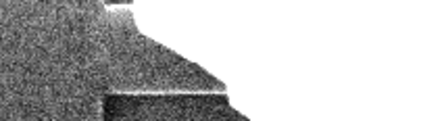
\includegraphics[width=0.31\textwidth]{5_Yield_Analysis/Fig/class_example_0.pdf}};
        \node at (0,-1.2) {\num{0}};
        \node[inner sep=0pt] (image) at (5.2,0) {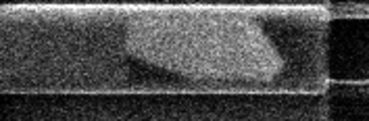
\includegraphics[width=0.31\textwidth]{5_Yield_Analysis/Fig/class_example_1.pdf}};
        \node at (5.2,-1.2) {\num{1}};
        \node[inner sep=0pt] (image) at (10.4,0) {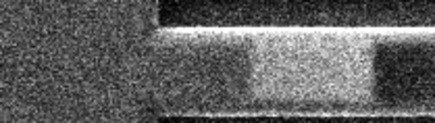
\includegraphics[width=0.31\textwidth]{5_Yield_Analysis/Fig/class_example_2.pdf}};
        \node at (10.4,-1.2) {\num{2}};
        \node[inner sep=0pt] (image) at (0,-3) {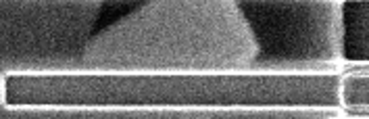
\includegraphics[width=0.31\textwidth]{5_Yield_Analysis/Fig/class_example_3.pdf}};
        \node at (0,-4.2) {\num{3}};
        \node[inner sep=0pt] (image) at (5.2,-3) {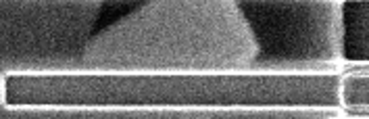
\includegraphics[width=0.31\textwidth]{5_Yield_Analysis/Fig/class_example_4.pdf}};
        \node at (5.2,-4.2) {\num{4}};
        \node[inner sep=0pt] (image) at (10.4,-3) {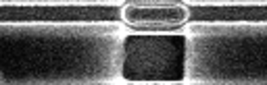
\includegraphics[width=0.31\textwidth]{5_Yield_Analysis/Fig/class_example_5.pdf}};
        \node at (10.4,-4.2) {\num{5}};
    \end{tikzpicture}
    \caption[Examples of each class of wire.]{Examples of each class of wire \cite{Brugnolotto2024}. The numbers below each image are the respective encodings, which can be interpreted from Table~\ref{tab:encodings}.}
    \label{fig:class_examples}
\end{figure}

\subsubsection{Digital image splitting algorithm}

\begin{figure}
    \centering
    \tikzsetnextfilename{raw_image}
    \begin{tikzpicture}
        \node[inner sep=0pt] (image) at (0, 0) {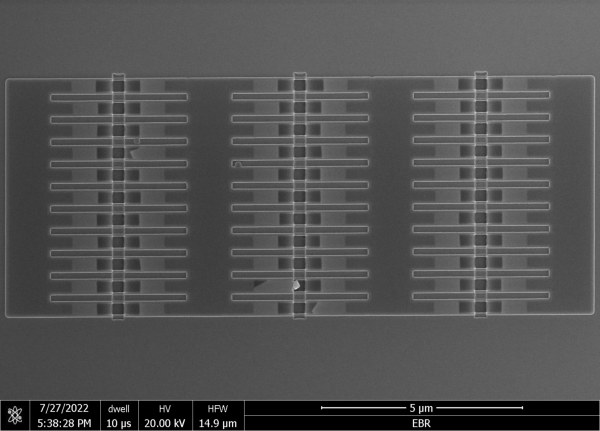
\includegraphics[width=\textwidth]{5_Yield_Analysis/Fig/raw_sem_image.pdf}};
        \draw[cb1_orange] (-7.5, -4) rectangle (7.5, 5);
        \node[anchor=north, cb1_orange] at (0, -4) {First cut};
        \draw[cb1_purple, dashed] (-7.5, -1) rectangle (7.5, 2);
        \node[anchor=west, cb1_purple, rotate=90] at (-7.2, -0.8) {Pooling area};
        \draw[cb1_light_blue] (-6.7, -2.8) rectangle (6.7, 3.85);
        \node[anchor=north, cb1_light_blue] at (0, -2.8) {Isolated array};
    \end{tikzpicture}
    \caption[An unprocessed \acs{sem_m} image of a nanowire array.]{A raw \acs{sem_m} image of a nanowire array. This is an example of the starting state of the images in the unprocessed dataset, in particular, this image has low contrast. The cutting process is also shown with rectangles of different colours.}
    \label{fig:raw_image}
\end{figure}

\begin{figure}
    \centering
    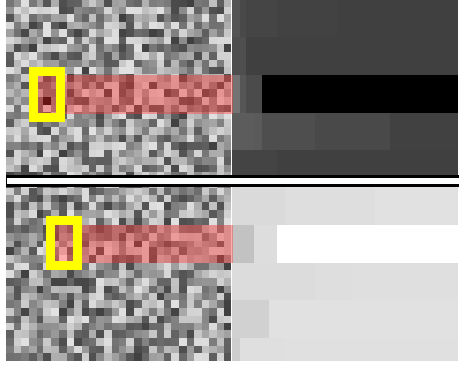
\includegraphics{5_Yield_Analysis/Fig/min_max_pool.pdf}
    \caption[Simpliefied example illustrating the operation of the \texttt{max\_pool} and \texttt{min\_pool} kernels.]{Simpliefied example illustrating the operation of the \texttt{max\_pool} and \texttt{min\_pool} kernels \cite{Brugnolotto2024}.}
    \label{fig:min_max_pool}
\end{figure}

The main challenge facing the creation of the input data set is to produce images of isolated nanowires from an image such as that in Figure~\ref{fig:raw_image}. This particular image was captured with low contrast; other images, such as those seen in Figure~\ref{fig:class_examples} were captured under different acquisition settings. The variety of acquisition conditions makes it challenging to define hardcoded intensity levels to, for example, detect whether or not a wire is there and what shape it has.

However, a constant for all images is the magnification and orientation, plus or minus some units of degree, of the nanowire arrays. Another constant is the information panel at the bottom of the image. While useful for human interpretation of the image, this part of the image is not necessary for a machine. Given its regular nature, it can be easily removed from all images by cutting a constant number of pixel rows. The geometry of the nanowire array remains constant as well, varying only in vertical size, with minor fluctuations in position inside the image.

Figure~\ref{fig:raw_image} shows the concept for the initial cutting steps. The first cut, highlighted in orange, using hard-coded coordinates, excludes the information panel at the bottom of the image and the nanowire array's left and right side walls. The coordinates of the next cut are computed on the basis of the relative intensities within a specific pooling area, represented by dashed purple lines. After four such operations, one per each side of the nanowire array, only the image data within the blue rectangle remain, and the nanowire array is therefore isolated.

Keeping track of the coordinates of the vertices of each cut is essential to correlate the label data in the \texttt{.json} file to the data in the image itself. The splitting algorithm uses the binary representation of the raw image contained in the \texttt{.json} label file to create a \texttt{numpy} \cite{Harris2020, numpy} array populated by \texttt{uint8} values. Each value gives the intensity of a pixel as an 8-bit unlabelled integer, which varies from \num{0} to \num{255}. Therefore, the resulting \texttt{numpy} array is the mathematical description of a black-and-white image. The data for all images are stored in its \texttt{numpy} array form in a variable inside a Python \texttt{class}, also containing its file name, label (once assigned) and coordinates relative to the raw image. These coordinates are kept updated throughout the image pre-processing steps.

\begin{sidewaysfigure}
    \centering
    \tikzsetnextfilename{pooling}
    \begin{tikzpicture}
        \node[inner sep=0pt, label={Denoised input}] (no_pool) at (0, 0) {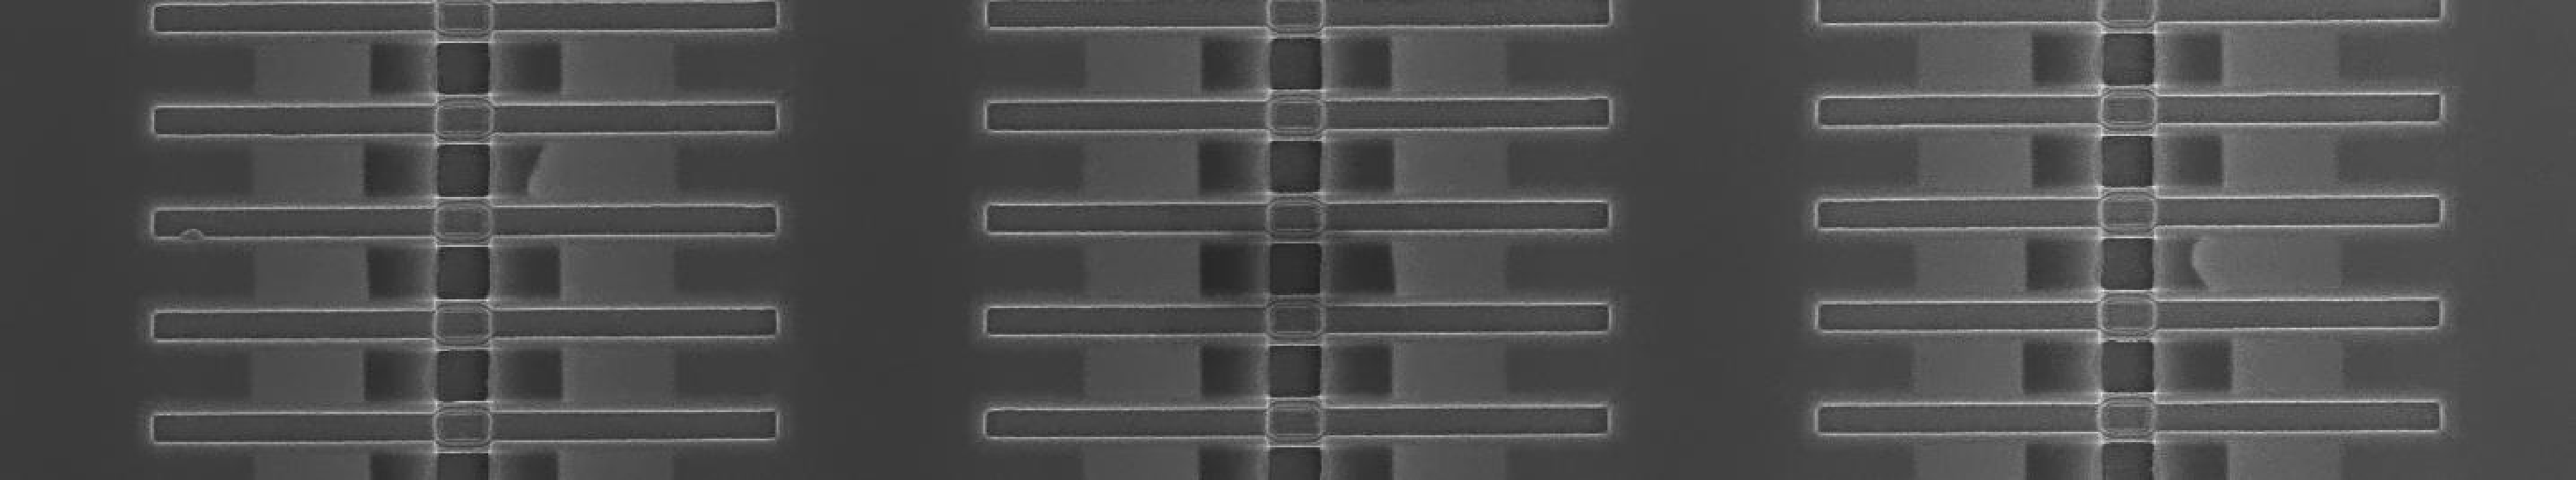
\includegraphics[width=0.4\textwidth]{5_Yield_Analysis/Fig/no_pool.pdf}};
        \node[inner sep=0pt] (max_pl) at (13, 0) {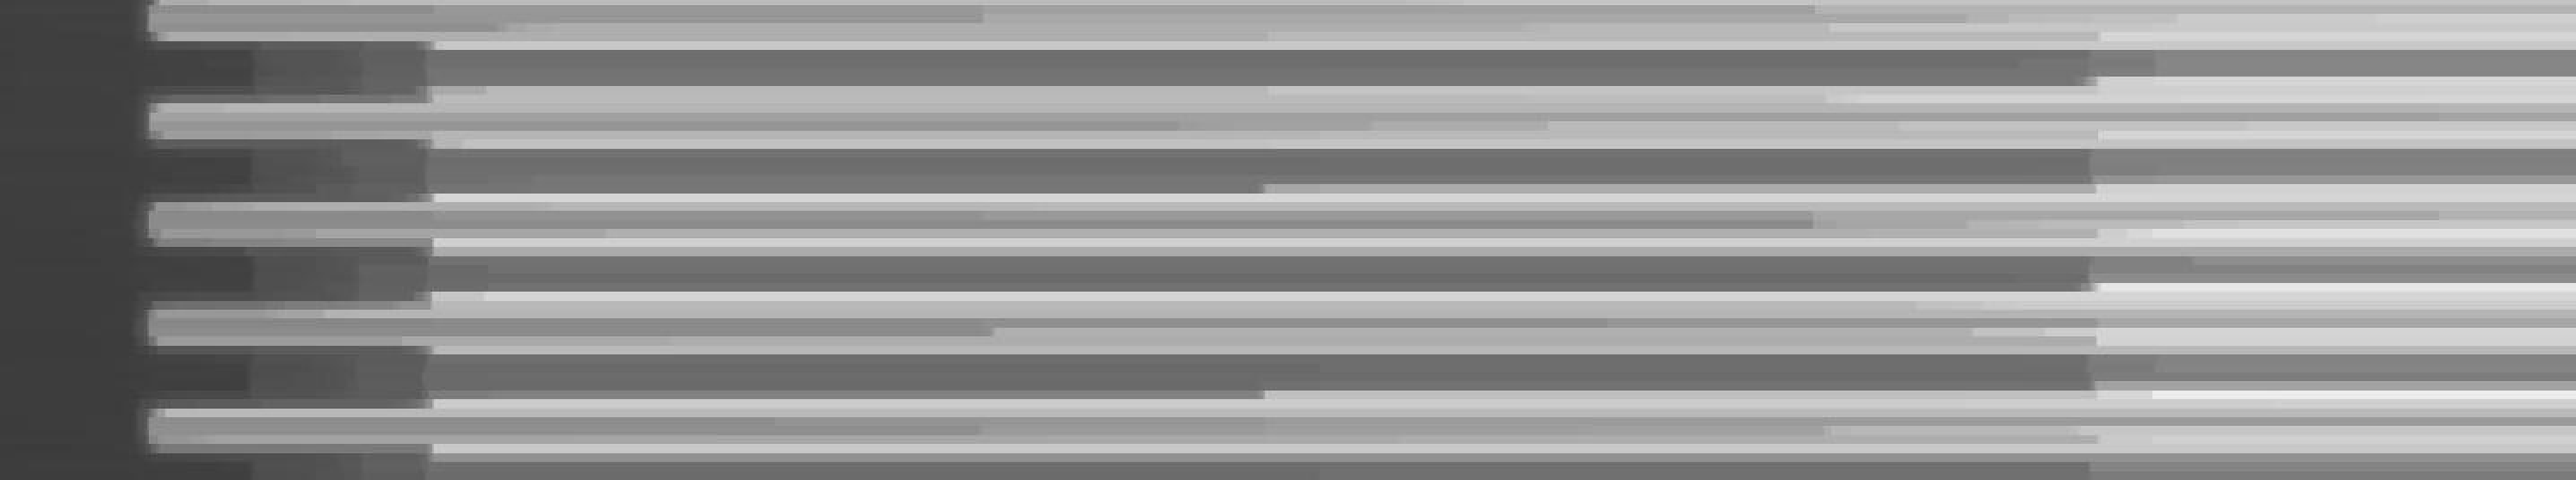
\includegraphics[width=0.4\textwidth]{5_Yield_Analysis/Fig/max_pl.pdf}};
        \node[inner sep=0pt] (min_pl) at (0, -4) {
\includegraphics[width=0.4\textwidth]{5_Yield_Analysis/Fig/min_pl.pdf}};
        \node[inner sep=0pt] (avg_max) at (13, -3) {
\includegraphics[width=0.4\textwidth]{5_Yield_Analysis/Fig/avg_max.pdf}};
        \node[inner sep=0pt] (avg_min) at (0, -7) {
\includegraphics[width=0.4\textwidth]{5_Yield_Analysis/Fig/avg_min.pdf}};
        \draw[-stealth] (no_pool) -- (max_pl) node[midway, anchor=south]{Max Pooling};
        \draw[-stealth] (max_pl) -- (avg_max) node[midway, anchor=west]{Vectorisation};
        \draw[-stealth] (no_pool) -- (min_pl) node[midway, anchor=west]{Min Pooling};
        \draw[-stealth] (min_pl) -- (avg_min) node[midway, anchor=west]{Vectorisation};
        \draw[-stealth] (avg_max.south) -- ++ (0, -1.5) node[midway, anchor=west]{Gradient};
        \draw[-stealth] (avg_min.east) -- ++ (2.8, 0) node[midway, anchor=south]{Gradient};
        \begin{axis}[%
            xshift= 9cm,
            yshift= -11cm,
            width = 9cm,
            xlabel = Position (pixel),
            ylabel = Gradient,
            table/col sep=comma,
            legend pos=north east,
            ymin=0, ymax=25,
            xmin = 0, xmax=1436
        ]
            \addplot [cb1_orange,] table[x=index,y=grad_max] {5_Yield_Analysis/csv/gradients.csv};
            \addplot [cb1_dark_blue,] table[x=index,y=grad_min] {5_Yield_Analysis/csv/gradients.csv};
            \addlegendentry{Max Pool Gradient}
            \addlegendentry{Min Pool Gradient}
        \end{axis};
    \end{tikzpicture}
    \caption[Max and min-pooling operations with vectorisation and gradient calculation for cut-point identification.]{Max and min-pooling operations with vectorisation and gradient calculation for cut-point identification.}
    \label{fig:pooling}
\end{sidewaysfigure}

The first hardcoded cut is performed by eliminating the first \num{100} and the last \num{200} \texttt{numpy} array rows and the first and last \num{50} \texttt{numpy} array columns. This operation eliminates the information panel at the bottom of the image and the bright lateral edges of the nanowire array, a step necessary to determine the exact cutting points. Figure~\ref{fig:pooling} shows how the precise image-cutting concept illustrated in Figure~\ref{fig:raw_image} is implemented. First, a copy of the image is made, and its top and bottom thirds are cut to isolate the pooling area and exclude the two remaining edges of the nanowire array. A denoising algorithm from the \texttt{opencv} library \cite{Bradski2000, opencv} was employed to eliminate pixels that, due to noise, might be too dark or too bright and, therefore, impact the detection of the correct edges with the pooling method.

The pooling method is based on two kernels parsing the \texttt{numpy} array and overwriting its values to highlight vertical edges. These kernels are called \texttt{min\_pool} and \texttt{max\_pool}. Aside from selecting either a minimum or maximum value, the implementation of the two kernels is identical. For brevity, the \texttt{max\_pool} method will be discussed. Intensity values within a box \num{5} pixels tall and \num{2} pixels wide are considered, and the maximum value is selected. Afterwards, the box is moved by one pixel to the right, and the procedure is repeated. Therefore, there is a \num{1} pixel of horizontal overlap so that if none of the \num{5} new pixels has a higher value than the ones in the previous box, the last high value is carried over. This box is horizontally moved starting at the top left of the image and, once the end of the rows is reached, is moved back to the beginning of the row and moved down by \num{5} pixels. As a result, there is no vertical carryover of values. A simplified example of the operation of these two kernels, with differently sized boxes, is shown in Figure~\ref{fig:min_max_pool}.

The resulting \texttt{numpy} arrays are visualised in Figure~\ref{fig:pooling}. Initially, the \texttt{max\_pool} and \texttt{min\_pool} operations were meant to identify the beginning and the end of the III-V segment. This is accomplished very well by the \texttt{min\_pool} operation. Thick dark lines can be seen in the \texttt{min\_pool} output starting at the position corresponding to the end of the leftmost III-V segments in the denoised input. Unfortunately, the result of the \texttt{max\_pool} is dominated by the internal template sidewalls of the nanowire array. 

This difference in outcome is the reason why the idea of isolating only the area of the image corresponding to the III-V nanowires was abandoned and, instead, the goal shifted to isolating the portion of seed, nanowire and empty templates together, as was shown in Figure~\ref{fig:class_examples}.

To determine the cut-point the \texttt{numpy} arrays resulting from the pooling operations were vectorised, as in, reduced to one-dimensional \texttt{numpy} arrays, by taking the maximum value, for the \texttt{max\_pool} output, or the minimum value, for the \texttt{max\_pool} output, of each column. The gradient of both vectors was then calculated using the \texttt{gradient} method of the \texttt{numpy} library, which returned the ratio of the variation in intensity to the variation in the position in the vector. The results of this operation for the image used as an example in this section are also shown in Figure~\ref{fig:pooling}.

During the development of the splitting algorithm, it was found that due to the shading in the \acs{sem_m} image both vectors had their largest gradients in the area corresponding to the introduction of the side walls of the comb tooth template. Furthermore, for the initial, smaller dataset used in the early trials, it was also found that taking the largest gradient further down the vector resulted in a tighter cut. Unfortunately, as seen in the plot in Figure~\ref{fig:pooling} this had to be changed in the code revisions carried out after the initial classifier training to include a handful of images for which the maximum gradient was much further after the desired cut point. In the first iterations of the splitting algorithm this would result in the image being excluded from the input dataset.

\begin{figure}
    \centering
    \subcaptionbox{
        Isolated nanowire array and division in columns.
        \label{subfig:wire_array}
    }{
        \tikzsetnextfilename{wire_array}
        \begin{tikzpicture}
            \node[inner sep=0pt] (image) at (0, 0) {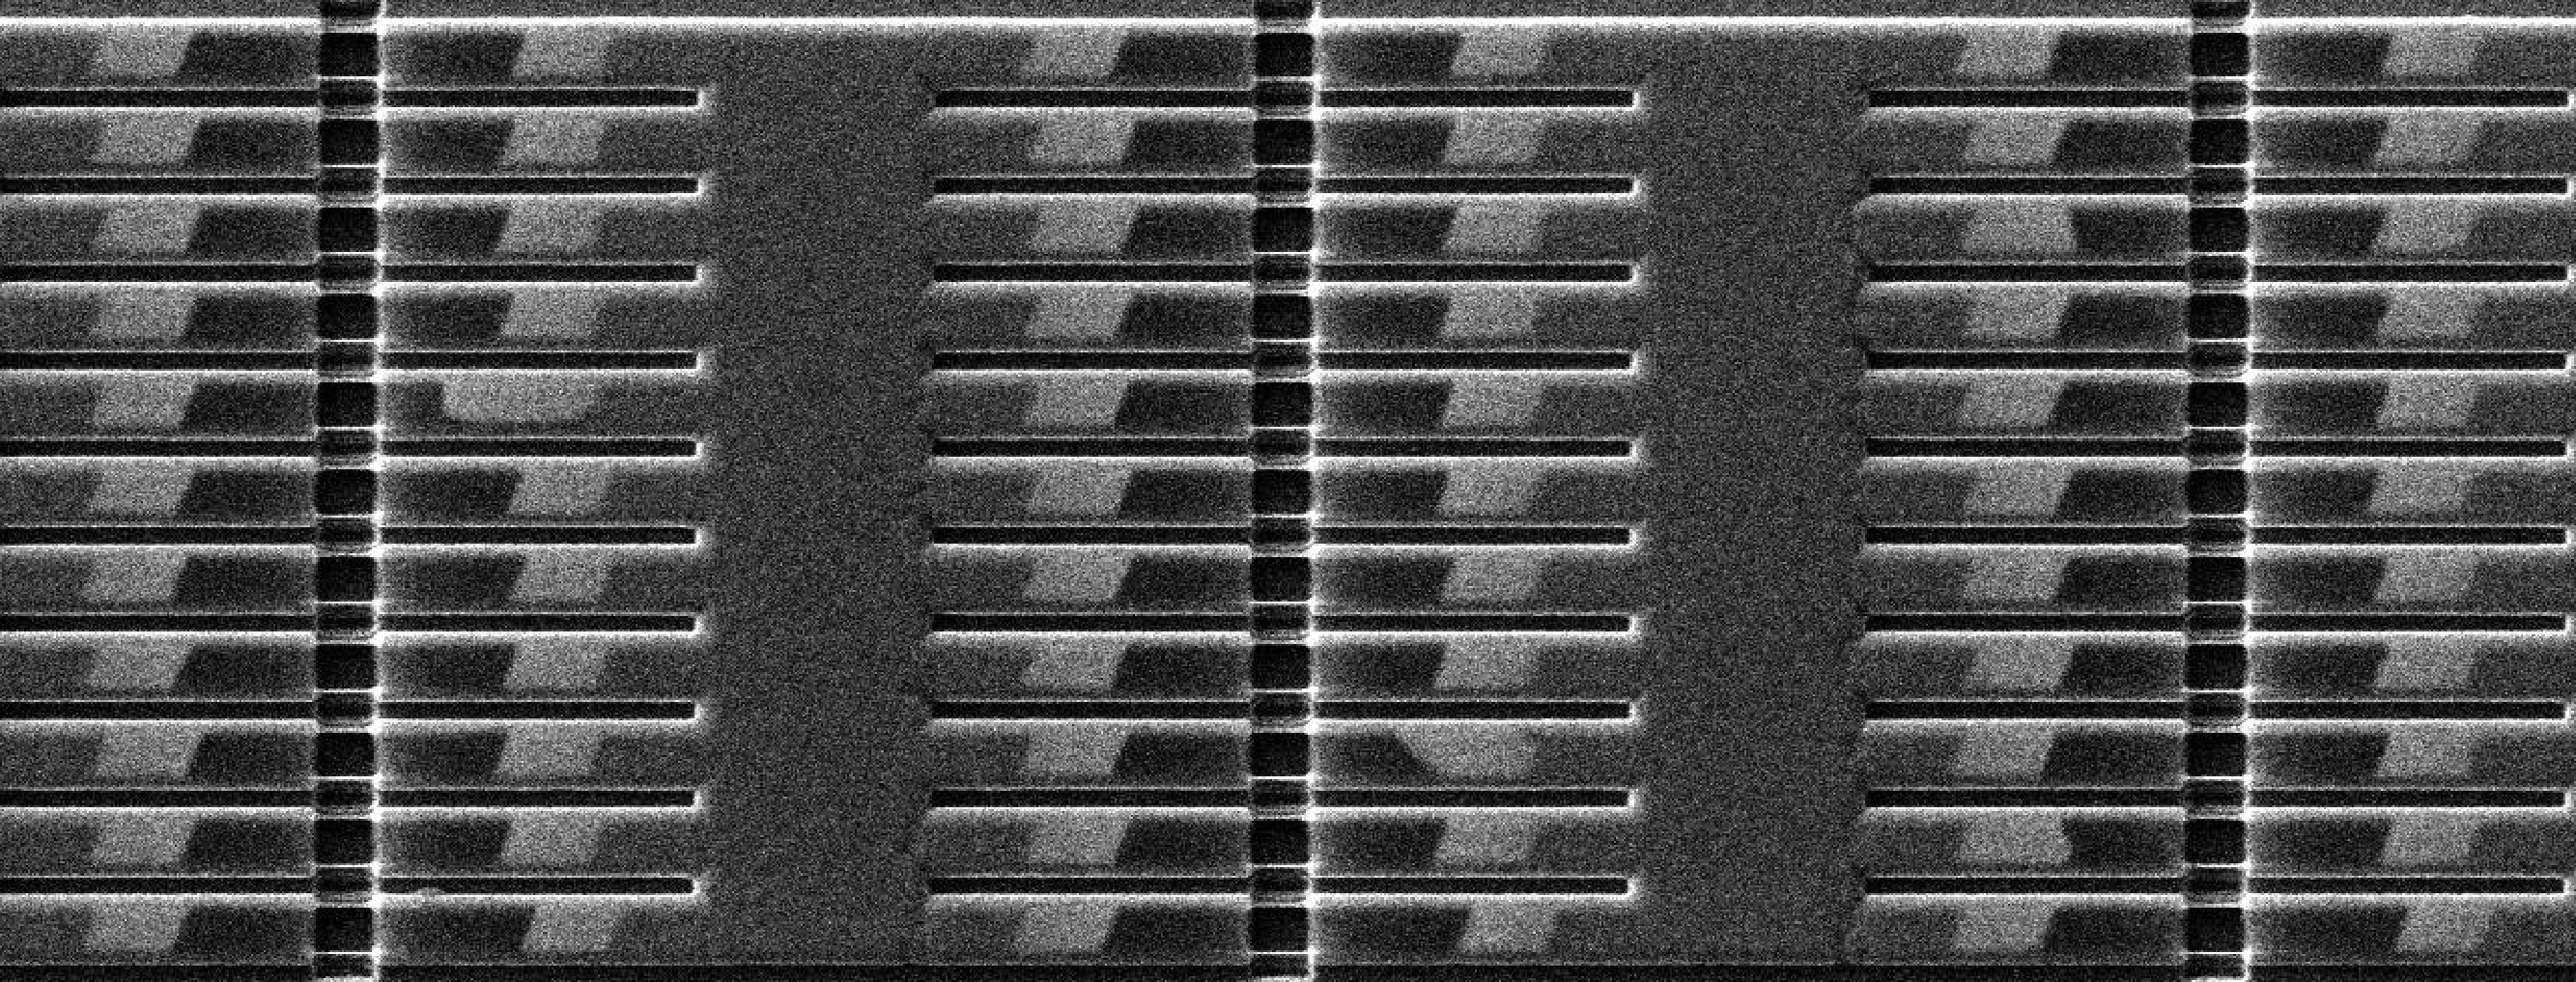
\includegraphics[width = 0.72\textwidth]{5_Yield_Analysis/Fig/wire_array.pdf}};
            \draw[cb1_light_blue, dashed] (-1.93333, -2.2) -- ++ (0, 4.4);
            \draw[cb1_light_blue, dashed] (1.93333, -2.2) -- ++ (0, 4.4);
        \end{tikzpicture}
    }
    \subcaptionbox{
        Final cuts
        \label{subfig:single_column_2}
    }{
        \tikzsetnextfilename{single_column_2}
        \begin{tikzpicture}
            \node[inner sep=0pt] (image) at (0, 0) {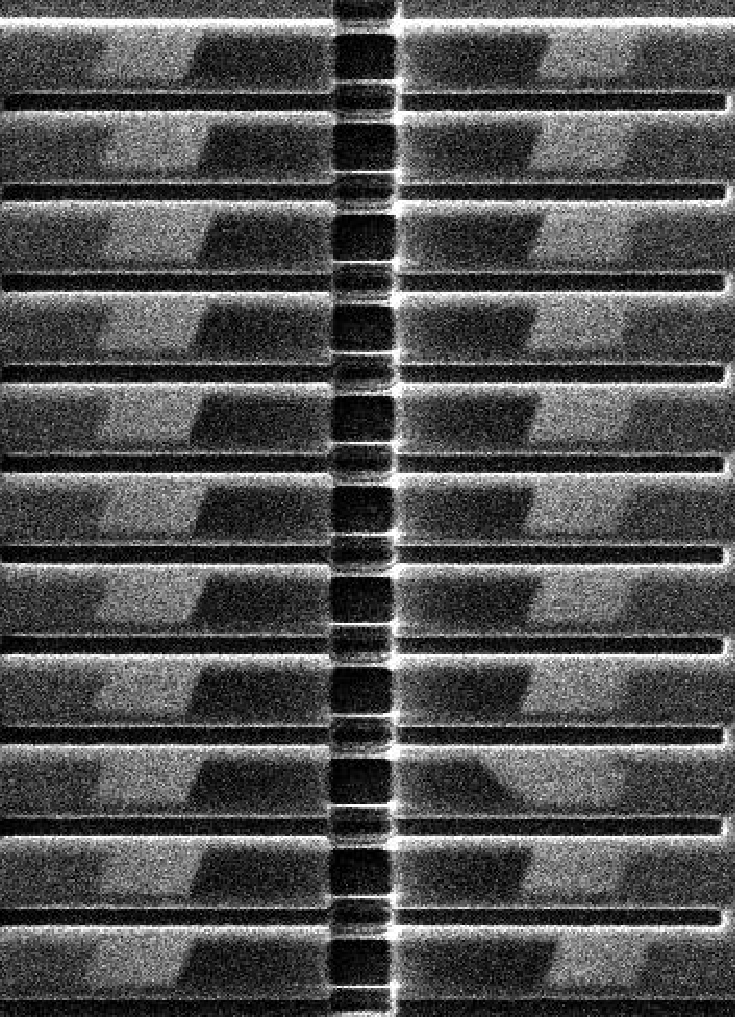
\includegraphics[width = 0.20\textwidth]{5_Yield_Analysis/Fig/single_column_2.pdf}};
            \draw[cb1_light_blue, dashed] (0, -2.25) -- ++ (0, 4.5);
            \foreach \y in {1, 2, 3, 4, 5, 6, 7, 8, 9, 10}
                \draw[cb1_orange, dashed] (-1.6, -2.25+\y*0.4091) -- ++ (3.2, 0);
        \end{tikzpicture}
    }
    \caption[Final cuts for the isolation of single wires.]{Final cuts for the isolation of single wires. \subref{subfig:wire_array} shows an image of a nanowire array as it appears after a successful cut with the method shown in Figure~\ref{fig:pooling}. The light blue dashed lines show the division in three equally sized parts picturing the three columns. \subref{subfig:single_column_2} shows a column after it has been reduced to the \num{22} wires, a light blue vertical line shows how the image is divided in two equally sized parts, while the 10 equally-spaced orange horizontal lines show the final subdivision into single wires.}
    \label{fig:fine_cutting}
\end{figure}

The procedure used to isolate this cut point is repeated after rotating the \texttt{numpy} array to calculate the cut points for all four sides of the nanowire array. The final result of these cutting operations is shown in Figure~\ref{subfig:wire_array}. The nanowire array is perfectly centred in this image, and the columns containing the nanowires can be split easily by dividing the image into three equally sized parts, as shown by the light blue dashed lines, resulting in three nanowire column images.

The remaining \acl{si} anchor areas in the nanowire array column images can be trimmed out with the same algorithm used to isolate the array (Figure~\ref{fig:pooling}), resulting in an image like that of Figure~\ref{subfig:single_column_2}, showing the central column of the nanowire array in Figure~\ref{subfig:wire_array} after refinement. By splitting this image in half vertically along the middle and then dividing the two halves horizontally in \num{11} equally-sized parts the single wires are isolated.

\subsubsection{Label assignment}

After completion of image splitting, each image must be assigned a label for supervised classifier training to take place. The coordinates of the position of the vertices delimitating each resulting image within the parent raw image were recorded throughout all transformation. They can be compared with the coordinates of the label saved in the \texttt{.json} file created by \texttt{labelme} during labelling.

To determine which label to assign to each refined image, the label list for the parent image is loaded and the coordinates of each point defining a label are checked to verify if they fall in the area corresponding to the refined image. When a label does it is added to a list. Ideally, the length of the list after all labels are processed should be \num{1}, only containing the label corresponding to the wire type (parallel or tilted) and growth result (perfect or defect). However, the splitting algorithm does not always result in the expected result, often due to the cut points being incorrect. This, plus some images containing two labels either due to nucleation on the internal template walls or parasitic III-V crystals growing on top of the nanowire array (as seen in Figure~\ref{fig:defects}) means that some images will have either \num{0} or more than \num{1}. 

\begin{table}
    \centering
    \caption[Percentages of each class in the input dataset after preprocessing with the original splitting algorithm.]{Percentages of each class in the input dataset after preprocessing with the original splitting algorithm.}
    \begin{tabular}{l|c|c c|c c|c}
        & & \multicolumn{2}{c|}{Wire Parallel} & \multicolumn{2}{c|}{Wire Tilted} & \\ 
        Class & Parasitic & Defect & Perfect & Defect & Perfect & Null \\ \hline \hline
        Percentage & \qty{1.8}{\%} & \qty{1.2}{\%} & \qty{25.8}{\%} & \qty{1.2}{\%} &\qty{18}{\%} & \qty{11.2}{\%}
    \end{tabular}
    \label{tab:class_makeup}
\end{table}

Images with \num{0} labels are removed from the input dataset and are not considered. Images with more than one label that do not contain a defective or parasitic label are assigned to the \texttt{Null} class. Conversely, if there is a defective or parasitic label, it is assigned to the image. Table~\ref{tab:class_makeup} shows the breakdown of the composition of the dataset resulting from the splitting algorithm in its first iteration. The percentages add up to \qty{59.2}{\%} as the remaining \qty{40.2}{\%} of images was incorrectly cut by the algorithm resulting in no matches with existing labels.

Aside from the flaws of the splitting algorithm, another issue is that the dataset is heavily unbalanced. The perfect wires dominate in quantity, having more than \num{10} times the number of defective wires. \qty{25.8}{\%} of the wires are parallel perfect, and \qty{18}{\%} are tilted perfect, reflecting very well the \qty{60}{\%} / \qty{40}{\%} split of the raw dataset between parallel and tilted arrays. Parallel and tilted defective wires make up an equal percentage (\qty{1.2}{\%}) of the splitting algorithm's output. \qty{1.8}{\%} of the output consists of images of parasitic crystals, and, finally, \qty{11.2}{\%} was assigned as \texttt{Null} class.

\subsection{Training}

\begin{figure}
    \centering
    \subcaptionbox{
        F1 score and loss for each training epoch \cite{Brugnolotto2024}.
        \label{subfig:F1Score}
    }{
        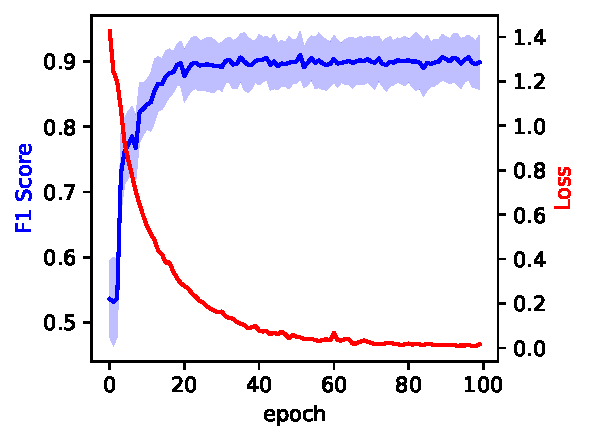
\includegraphics[width=0.48\textwidth]{5_Yield_Analysis/Fig/F1Score.pdf}
    }
    \subcaptionbox{
        Confusion Matrix of the classifier \cite{Brugnolotto2024}.
        \label{subfig:confusion_matrix}
    }{
        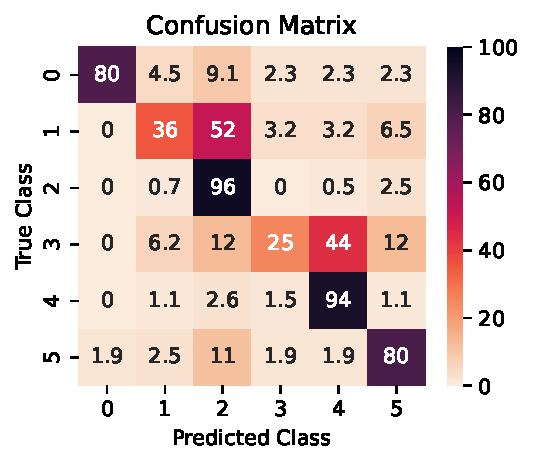
\includegraphics[width=0.48\textwidth]{5_Yield_Analysis/Fig/Confusion_Matrix.pdf}
    }
    \caption[Training metrics for the classifier.]{Training metrics for the classifier \cite{Brugnolotto2024}. \subref{subfig:F1Score} shows the evolution of the F1 score and the loss during training. \subref{subfig:confusion_matrix} shows the confusion matrix of the trained classifier calculated on the test fraction.}
    \label{fig:training_metrics}
\end{figure}

A compact model consisting of two convolutional layers, followed by three linear layers and based on the \texttt{pytorch} \cite{NEURIPS2019_9015, pytorch} framework was chosen. This simple model showed good performance when classifying commonly used datasets, such as CIFAR-10 \cite{NIPS2012_c399862d}. The input dataset as resulting from the splitting algorithm and label assignment was divided into a training set, comprising \qty{70}{\%} of the data, and a validation set containing the remaining \qty{30}{\%}. The sets were filled with random images, respecting the original composition of the dataset.

The three metrics of loss, F1 score, and confusion matrix were used to evaluate the classifier's performance \cite{grandini2020}. The cross-entropy loss function, integrated with the Adam algorithm, was used to guide the learning process \cite{Brugnolotto2024}.

The classifier was trained until loss saturation was achieved, a process that lasted \num{100} epochs. The red curve in Figure~\ref{subfig:F1Score} shows the saturation process, with loss, shown on the y-axis on the right side, reaching \num{0} at the end of the \num{100} training epochs. The blue line in Figure~\ref{subfig:F1Score} shows the evolution of the F1 score during training, with the shaded area around it representing the \qty{97}{\%} confidence interval on this metric.

The best classifier achieved an F1 score of \num[separate-uncertainty=true]{0.91 (4)} (\qty{97}{\%} confidence interval), as calculated on the test fraction. However, this metric alone is insufficient to properly assess the performance of the classifier given the very high imbalance in the dataset. 

The confusion matrix in Figure~\ref{subfig:confusion_matrix} provides a much clearer assessment of the class-specific performance of the classifier. The diagonal elements (top left to bottom right) of this matrix represent the recall, the ratio of true positives to the sum of true positives and false negatives, as a percentage. The higher the recall for each class the better the classifier is at assigning the correct class to an image. Therefore, the classifier does a very good job at classigying images containing parasitic crystals, perfect parallel and tilted wires, and \texttt{Null} images. These four classes have recalls of \qty{80}{\%} or higher, with wire perfect classes showing a recall of \qty{96}{\%} and \qty{94}{\%} for parallel and tilted wires, respectively. The defective classes, however, have very low recalls, with perfect parallel wires correctly identified only \qty{36}{\%} of the time and their tilted counterparts only \qty{25}{\%} of the time. When the off-diagonal components of the confusion matrix are examined, it is easily seen that defective wires are more often than not incorrectly classified as perfect. This is likely due to the disproportionate prevalence of perfect wires, but also to the relatively minor visible alteration of some of the defective wires compared to their perfect counterparts.

Collecting more images of defective wires is therefore a necessary step to create a more balanced input set and improve the recall of defective classes. It is worth noting that, despite the splitting algorithm's mixed success in properly processing half of the raw dataset, the classifier still managed to assign four out of six classes with very high accuracy.

\subsection{Improvements to the digital image splitting algorithm}

\begin{table}
    \centering
    \caption[Percentages of each class in the input dataset after preprocessing with the revised splitting algorithm.]{Percentages of each class in the input dataset after preprocessing with the revised splitting algorithm.}
    \begin{tabular}{l|c|c c|c c|c}
        & & \multicolumn{2}{c|}{Wire Parallel} & \multicolumn{2}{c|}{Wire Tilted} & \\ 
        Class & Parasitic & Defect & Perfect & Defect & Perfect & Null \\ \hline \hline
        Percentage & \qty{2.6}{\%} & \qty{1.5}{\%} & \qty{35.9}{\%} & \qty{1.2}{\%} &\qty{24.4}{\%} & \qty{0}{\%}
    \end{tabular}
    \label{tab:class_makeup2}
\end{table}

Changes were made to make the \texttt{ Null} class unnecessary by allowing the algorithm to discriminate between multiple labels on the same image. This was done by computing the area of the intersections of each label polygon with the images using the \texttt{shapely} \cite{gillies_2024} library. The label with the highest intersection area is then assigned to the image.

Another change concerned the cut-point determination in the algorithm shown in Figure~\ref{fig:pooling}. The algorithm was changed to only process each image with the \texttt{max\_pool} kernel and calculate the associated vectors and gradient. This solved the issue of the wrong point being chosen due to the influence of the \texttt{min\_pool} kernel discussed in previous sections.

The results of these two modifications are shown in Table~\ref{tab:class_makeup2}. Only \qty{34.4}{\%} of the raw dataset is marked for deletion in this version of the splitting algorithm. It is worth noting, however, that the classes that benefit the most from these modifications are the wire perfects. Indeed, while the wire parallel defect class gained \qty{0.3}{\%} more share of the raw dataset, the wire parallel perfect class gained \qty{10.1}{\%}. Similarly, the share of wire tilted defect class stays unchanged, while the wire tilted perfect increases by \qty{6.4}{\%}. These new results, coupled with the high recall for the \texttt{Null} class, point to the original splitting algorithm being already sufficiently apt for the task of creating a dataset to train a classifier.

\section{Discussion and future directions}

This chapter explored the yield statistics for the \hkl{1 1 1} growth front stabilisation method introduced and developed in Chapters~\ref{chap:growth} and \ref{chap:properties}. The survey carried out on \num{15840} nucleation sites across \num{240} nanowire arrays found a global yield of \qty{92.55}{\%} \cite{Brugnolotto2023_2}. It also highlighted the three most common defects, which were wires that grew with the wrong facet, totalling \num{368} wires or \qty{31.19}{\%} of defective sites, short wires, \num{211} or \qty{17.88}{\%} of defective sites, and the highest defect category: growth sites hidden by parasitic crystals with \num{487} sites or \qty{41.27}{\%} of defective sites. The number of wires hidden by parasitic crystals is so high that if they were excluded from the yield calculation, the total yield would grow by \qty{2.77}{\%} to \qty{95.32}{\%}.

Nucleation-related issues represented two-thirds (\num{796} or \qty{67.46}{\%}) of the recorded defects, mostly due to surface treatment-related issues, such as loss of selectivity and seed surface conditions. This points to the strength of the facet stabilisation method as a reliable and controlled approach to the growth of monolithically integrated III-V crystals on chip-sized surfaces, supplementing observations on a more local level regarding the merging of multiple crystals in a single structure shown in Section~\ref{sec:merge}.

The survey of the two samples that resulted in the statistical data on growth yield also produced a labelled dataset containing \num{240} \acs{sem_m} images \cite{dataset}, publicly available for use under the CC BY 4.0 licence \cite{CCBY40}. In this chapter, the dataset was used to train a classifier that could distinguish between the two orientations of the nanowire arrays. The classifier achieved good performance in discriminating perfect wires between tilted and parallel but struggled with the identification of defective wires. This can be attributed to the high imbalance in the dataset, which can be resolved by collecting more images of defective wires of both kinds to supplement the currently available data. Further improvements can also be made to the wire-splitting algorithm, where a different approach might yield a more reliable solution to the determination of the cut points.










% \section{article2}
% \begin{figure}
%     \centering
%     \includegraphics[width=\textwidth]{4_Properties/From_Article2/Figure2.png}
%     \caption{Top-view SEM images of arrays with grown III-V nanowires. The \qty{70}{\nm}, \qty{140}{\nm}, \qty{210}{\nm}, and \qty{280}{\nm} wide wires are shown from top to bottom. The arrays on the left contain structures grown from a seed surface parallel to the template direction, while those on the right are grown from seed surfaces that are tilted concerning the template. On the bottom left of the images, the three main elements of the arrays are highlighted in green (silicon seed), red (III-V nanowires), and blue (template opening).}
%     \label{fig:arrays}
% \end{figure}

% Figure~\ref{fig:arrays} shows growth results from sample 1 of arrays containing template nanotubes of four different widths (\qty{70}{nm}, \qty{140}{nm}, \qty{210}{nm}, and \qty{280}{nm}). Each array contains 66 nanowires (in red) grown from silicon (in green) and arranged in 33 pairs. Each pair of wires shares the same template opening (in blue). 
% \par
% Each wire in the array can be identified by its row, opening, and position relative to the latter. Each row is numbered from 1 to 11, starting at the bottom of the array. The template openings are marked by letters A, B, or C; the wires connected to the opening to the left (l) or right (r) can be easily distinguished. Therefore, a string such as 9Br identifies a single wire in the array. 
% \par
% Our growth methodology aims to select and maintain a single \hkl{111}\(_B\) facet as the nanowire's growth front. If a III-V wire end-surface is multi-faceted or not parallel to the \acs{si} seed facet, the wire is classified as defective in this study without requiring a further in-depth STEM analysis. This first distinction allows the evaluation of the fraction of "perfect" wires, defining a growth yield. 
% \par
% In Figure~\ref{fig:arrays}, the \qty{280}{nm} tilted arrays present some defective wires in 11Al, 6Cr, and 7Cr; however, the other wires in each pair (11Ar, 6Cl, and 7Cl) appear “perfect”. As is evident in the case of wire 6Cr, the wire grew into an unpredictable shape after nucleation. It is unclear if the source of defective wires can be attributed solely to the nucleation step, as there are other sites (\qty{70}{nm} tilted 6Cl, \qty{140}{nm} perpendicular 2Br, 11Br, and \qty{280}{nm} perpendicular 7Br) that present a defective wire and fully covered seed. However, this finding suggests that nucleation does play an important role in the following growth facet selection.


% \begin{figure}
%     \centering
%     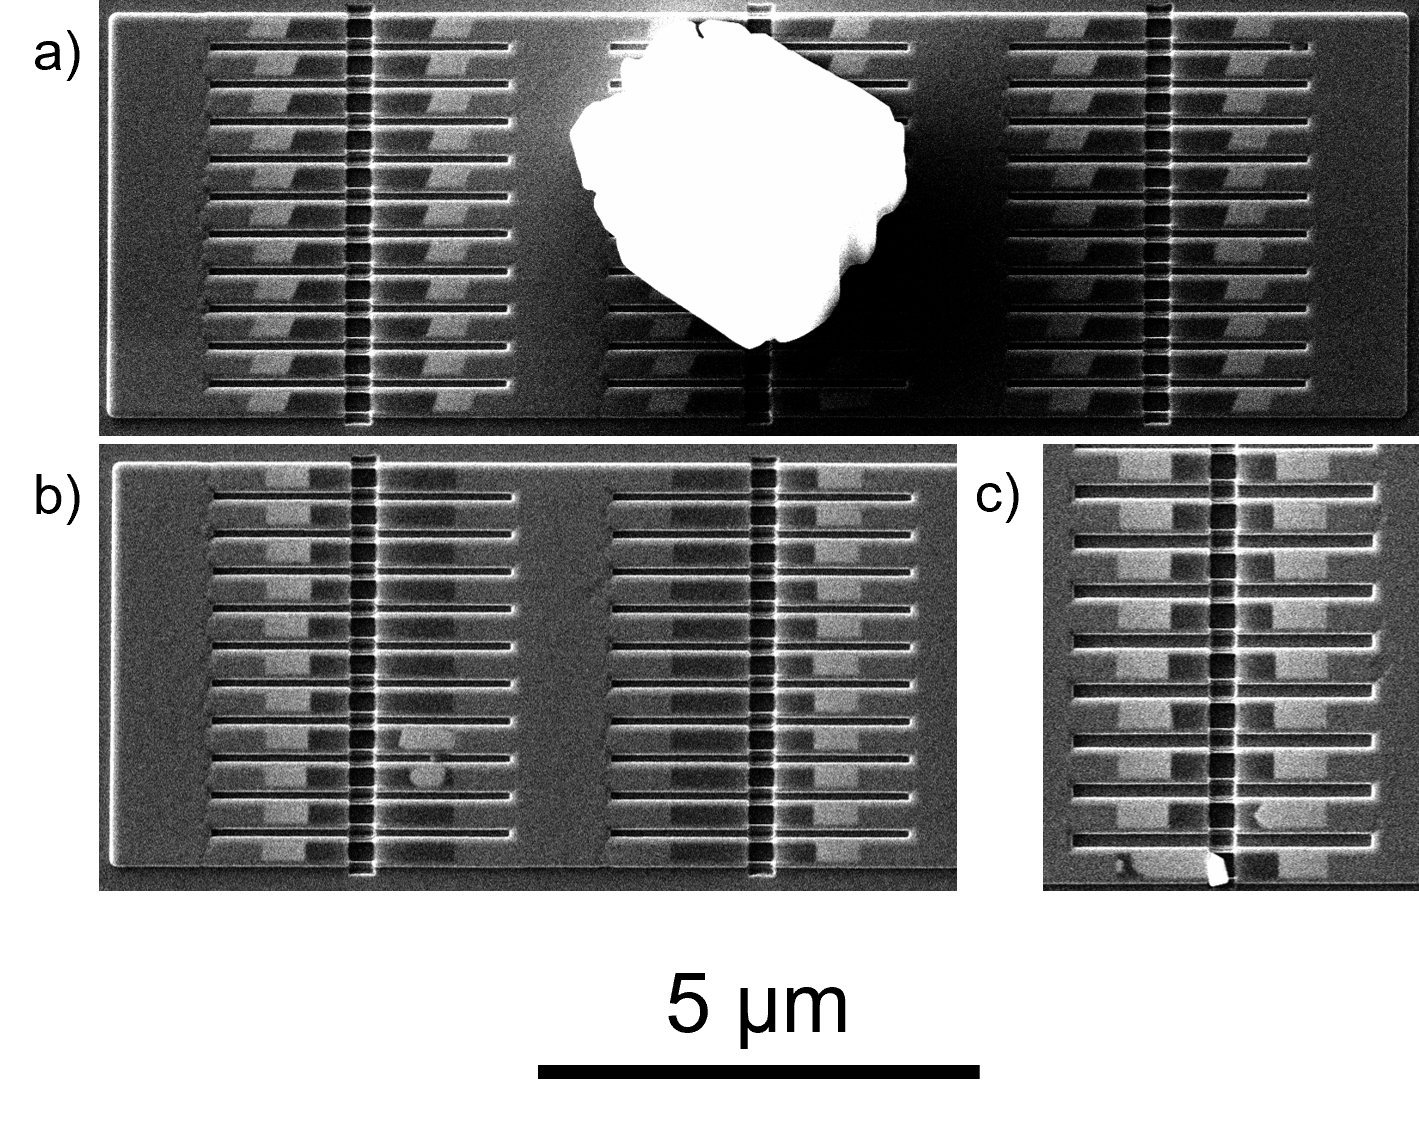
\includegraphics[width=\columnwidth]{4_Properties/From_Article2/Figure3.png}
%     \caption{Examples of failure situations for TASE grown wires. (a) large parasitic crystal obstructing many growth sites. (b) multiple seeds do not show nucleation of III-V material at all, while one site shows parasitic nucleation inside the template. (c) in the bottom row, after initial nucleation on the \acs{si}, a parasitic crystal developed inside the template and grew out of it.}
%     \label{fig:failures}
% \end{figure}

% Another parameter that negatively affects the growth yield is the loss of growth selectivity and the resulting parasitic growth. This is ascribed to impurities or surface features promoting nucleation. An example of this is shown in Figure~\ref{fig:defects}.a, where a single defect of this kind affects many wires. Figure~\ref{fig:defects}.b also shows sites where parasitic nucleation occurred within templates and, seed-sites that did not undergo III-V on \acs{si} nucleation, likely because of the lingering of a passivating \acs{sio2} layer on the \acs{si} seed surface. This happened despite the proximity to other correctly-grown wires. Finally, 
% Figure~\ref{fig:defects}.c bottom row illustrates an example where, after the initial nucleation event, the channel was obstructed by a parasitic nucleation growth within the channel, which extends outside the template. This type of growth configuration can potentially cause deposits similar to that in Figure~\ref{fig:defects}.a.

% \subsection{Yield study}

% \begin{table}
%     \centering
%     \caption[Overview of the distribution of defect types for samples 1 and 2.]{Overview of the distribution of defect types for samples 1 and 2 \cite{Brugnolotto2023_2}.}
%     \begin{tabular}{l|ccccccc}
%         \hline
%          & \multicolumn{7}{c}{Defect categories and occurrence} \\ 
%          & $\begin{matrix} \text{Wrong} \\ \text{Facet} \end{matrix}$ & $\begin{matrix} \text{Hidden by} \\ \text{Parasitic} \end{matrix}$ & $\begin{matrix} \text{Oxide} \\ \text{Nucleated} \end{matrix}$ & $\begin{matrix} \text{Seed} \\ \text{Exposed} \end{matrix}$ & Long & Short & Ungrown \\ 
%         \hline \hline
%          & & & & & & & \\
%         Sample 6 & \num{164} & \num{230} & \num{2} & \num{0} & \num{5} & \num{204} & \num{61} \\ 
%         \hline
%         Parallel & \num{81} & \num{170} & \num{1} & \num{0} & \num{4} & \num{0} & \num{0} \\
%         \textit{\% of category} & \textit{\qty{49.4}{\%}} & \textit{\qty{77.9}{\%}} & \textit{\qty{50}{\%}} & \textit{-} & \textit{\qty{80}{\%}} & \textit{\qty{0}{\%}} & \textit{\qty{0}{\%}} \\ 
%         \hline
%         Tilted & \num{83} & \num{51} & \num{1} & \num{0} & \num{1} & \num{204} & \num{61} \\
%         \textit{\% of category} & \textit{\qty{50.6}{\%}} & \textit{\qty{22.1}{\%}} & \textit{\qty{50}{\%}} & \textit{-} & \textit{\qty{20}{\%}} & \textit{\qty{100}{\%}} & \textit{\qty{100}{\%}} \\ 
%         \hline
%          & & & & & & & \\
%         Sample 7 & \num{204} & \num{257} & \num{15} & \num{8} & \num{3} & \num{7} & \num{20} \\ 
%         \hline
%         Parallel & \num{127} & \num{145} & \num{6} & \num{4} & \num{1} & \num{5} & \num{20} \\
%         \textit{\% of category} & \textit{\qty{62.3}{\%}} & \textit{\qty{56.4}{\%}} & \textit{\qty{40}{\%}} & \textit{\qty{50}{\%}} & \textit{\qty{33.3}{\%}} & \textit{\qty{71.4}{\%}} & \textit{\qty{100}{\%}} \\ 
%         \hline
%         Tilted & \num{77} & \num{112} & \num{9} & \num{4} & \num{2} & \num{2} & \num{0} \\
%         \textit{\% of category} & \textit{\qty{37.7}{\%}} & \textit{\qty{43.6}{\%}} & \textit{\qty{60}{\%}} & \textit{\qty{50}{\%}} & \textit{\qty{66.7}{\%}} & \textit{\qty{28.6}{\%}} & \textit{\qty{0}{\%}} \\ 
%         \hline
%         & & & & & & & \\
%         \textbf{Total} & \textbf{\num{368}} & \textbf{\num{487}} & \textbf{\num{17}} & \textbf{\num{8}} & \textbf{\num{8}} & \textbf{\num{211}} & \textbf{\num{81}} \\
%         \hline
%     \end{tabular}
%     \label{tab:defects}
% \end{table}

% A survey of the arrays was carried out using samples 1 and 2, and involved \num{15840} individual nanowires grown in \num{240} arrays grouped in \num{5} locations per sample. The areas investigated were the top left of the chips as well as randomly selected locations throughout it. Wires need to have two parallel visible \hkl{111} seed and end facets of equal length, and they need to have nucleated directly on the \acs{si} seed covering it in its entirety for them to be considered "perfect". Of the \num{15840} total wires \num{14660} match these criteria, totalling a global yield of \qty{92.55}{\%}.
% \par
% Of the \num{7920} wires imaged for each sample, \num{7254} grew successfully in sample 1, and \num{7406} grew successfully in sample 2, resulting in a corresponding growth yield of \qty{91.59}{\%} and \qty{93.51}{\%}. This result indicates that the different heterointerfaces of samples 1 and 2 do not significantly impact the growth yield. 
% \par
% Further analysis was carried out within each sample by comparing the template growth yield parallel to the \hkl<111> direction, and those tilted away from it. A larger number (\num{9504} out of \num{15840}) of wires of the first configuration were measured. For sample 2, the parallel and tilted configurations resulted in comparable growth yields of \qty{93.73}{\%} and \qty{93.75}{\%}, while sample 1 showed \qty{94.84}{\%} and \qty{86.71}{\%} growth yields for the same configurations. The larger difference in growth yields for parallel and tilted templates in sample 1 can be explained by one of the fivcategorisedselected locations containing tilted arrays, falling in an area of the chip with many nucleation issues. This area is reflected in Table~\ref{tab:failures} where sample 1 has more short and ungrown wires.
% \par
% The total of \num{1180} nanowires that experienced growth failure are categorised based on the type of failure they experienced. Table~\ref{tab:failures} breaks down the number of defective wires for each sample between parallel and tilted templates, on a per-category basis. The first category, labelled "wrong facet", groups wires which terminate with either a multi-faceted surface or in a single facet that is not parallel to the seed surface, and accounts for \num{368} wires (\qty{31.2}{\%} of the total defective wires). The second and largest category comprises wire locations hidden by a parasitic crystal (\num{461} wires or \qty{39.0}{\%} of the total failures). From a total of \num{240} arrays, \num{32} are affected by one or more parasitic crystals. Still, the parasitic crystals hide close to \num{15} (\num{14.87} on average) locations for nanowire growth in each of these arrays. The "oxide nucleated" category contains all the cases where a III-V crystal nucleated randomly inside a template instead on the \acs{si} seed and counts \num{17} wires, \qty{1.4}{\%} of the total. The wires in the category "seed exposed" have the expected end facet, but did not fully cover the entire seed surface, leaving some of it exposed (\num{8} wires, \qty{0.7}{\%}). The category "long" comprises wires that were significantly longer than the others but did not have other defects, accounting for \qty{0.7}{\%} of the defective wires for a total of \num{8}. The last two categories are abnormally short wires and ungrown wires, with \num{211} (\qty{20.1}{\%}) and \num{81} (\qty{6.9}{\%}) counts each. These two categories of wires are more common in the area which presented nucleation iCharacterisation1.